\documentclass{mcmthesis}
\mcmsetup{
	CTeX = false,
	tcn = {2504496},
	problem = \textcolor{red}{A},
	sheet = true,
	titleinsheet = true,
	keywordsinsheet = true,
	titlepage = false,
	abstract = false
}

\usepackage{tcolorbox}
\usepackage{xcolor}
\usepackage{adjustbox} % 在导言区添加
\definecolor{customblue}{RGB}{165,216,255} % 定义 #a5d8ff 的 RGB 值
\definecolor{deepblue}{RGB}{0,74,173}      % 配套深蓝色

% ================ 环境定义 ================
\newenvironment{featurebox}[1]{%
	\begin{tcolorbox}[
		colback=white,                  % 白色背景
		colframe=customblue,            % 边框颜色 #a5d8ff
		colbacktitle=customblue,        % 标题背景色
		coltitle=deepblue,              % 标题文字颜色
		arc=3mm,                        % 圆角半径
		boxrule=1.5pt,                  % 边框粗细
		title={\large\bfseries #1},     % 标题内容
		fonttitle=\sffamily,            % 无衬线字体
		top=10pt,                       % 上边距
		bottom=10pt,                    % 下边距
		left=10pt,                      % 左边距
		right=10pt,                     % 右边距
		]
	}{\end{tcolorbox}}
% ================ 预声明hyperref选项 ================
\PassOptionsToPackage{hyphens}{url}
\PassOptionsToPackage{colorlinks=true, linkcolor=blue, urlcolor=cyan, citecolor=magenta}{hyperref}

% ================ 基础包配置 ================
\usepackage{newtxtext}
\usepackage{amsmath}
\usepackage{graphicx}
\usepackage{tabularx}
\usepackage{array}
\usepackage{booktabs}
\usepackage[table,xcdraw]{xcolor}

% ================ 算法排版包 ================
\usepackage{algorithm}
\usepackage{algpseudocode}

% ================ 参考文献配置 ================
\usepackage[style=ieee,backend=biber]{biblatex}
\addbibresource{reference.bib}

% ================ 目录格式配置 ================
\usepackage{tocloft}
\setlength{\cftbeforesecskip}{6pt}
\renewcommand{\contentsname}{\hspace*{\fill}\Large\bfseries Contents \hspace*{\fill}}

% ================ 页眉页脚配置 ================
\usepackage{fancyhdr}
\setlength{\headheight}{13.6pt}

% ================ 子图表支持 ================
\usepackage{subcaption}

% ================ 最后加载hyperref ================
\usepackage{hyperref} % 必须保持最后加载

% ================ 自定义颜色 ================
\definecolor{lightgray}{RGB}{240,240,240}
\definecolor{lightblue}{RGB}{173,216,230}

% ================ 表格样式配置 ================
\newcolumntype{Y}{>{\raggedright\arraybackslash}X}
\setlength{\arrayrulewidth}{0.5mm}
\setlength{\tabcolsep}{12pt}
\renewcommand{\arraystretch}{1.2}

\title{Enjoy a Cozy and Green Bath}
\date{\today}
\begin{document}
	
	%%%%%%%%%%%%%%%%%%%%%%%%%%%%%%%%%%%%%%%%
	%%%%%%%%%%%%%%%%% 摘要 %%%%%%%%%%%%%%%%%
	%%%%%%%%%%%%%%%%%%%%%%%%%%%%%%%%%%%%%%%%
	\begin{abstract}
		
		abstract...
		
		\begin{keywords}
			Keyword one, Keyword two, Keyword three
		\end{keywords}
		
	\end{abstract}
	
	
	\maketitle
	\tableofcontents        % 若不想要目录, 注释掉该句
	\thispagestyle{empty}
	\newpage
	
	
	
	
	
	%%%%%%%%%%%%%%%%%%%%%%%%%%%%%%%%%%%%%%%%
	%%%%%%%%%%%%%%%%% 引言 %%%%%%%%%%%%%%%%%
	%%%%%%%%%%%%%%%%%%%%%%%%%%%%%%%%%%%%%%%%
	
	
	\section{Introduction}
	
	\subsection{Background}
	The medal table of the 2024 Paris Olympics shows that the United States and China each won 40 gold medals and tied for the top spot, but the United States led with a total of 126 medals. The host country France ranked fifth in gold medals (16) and fourth in total medals (64). Dominica, Saint Lucia and other countries won their first Olympic medals, while 60 countries still have not broken through for any medals.
	\begin{figure}[htbp]
		\centering
		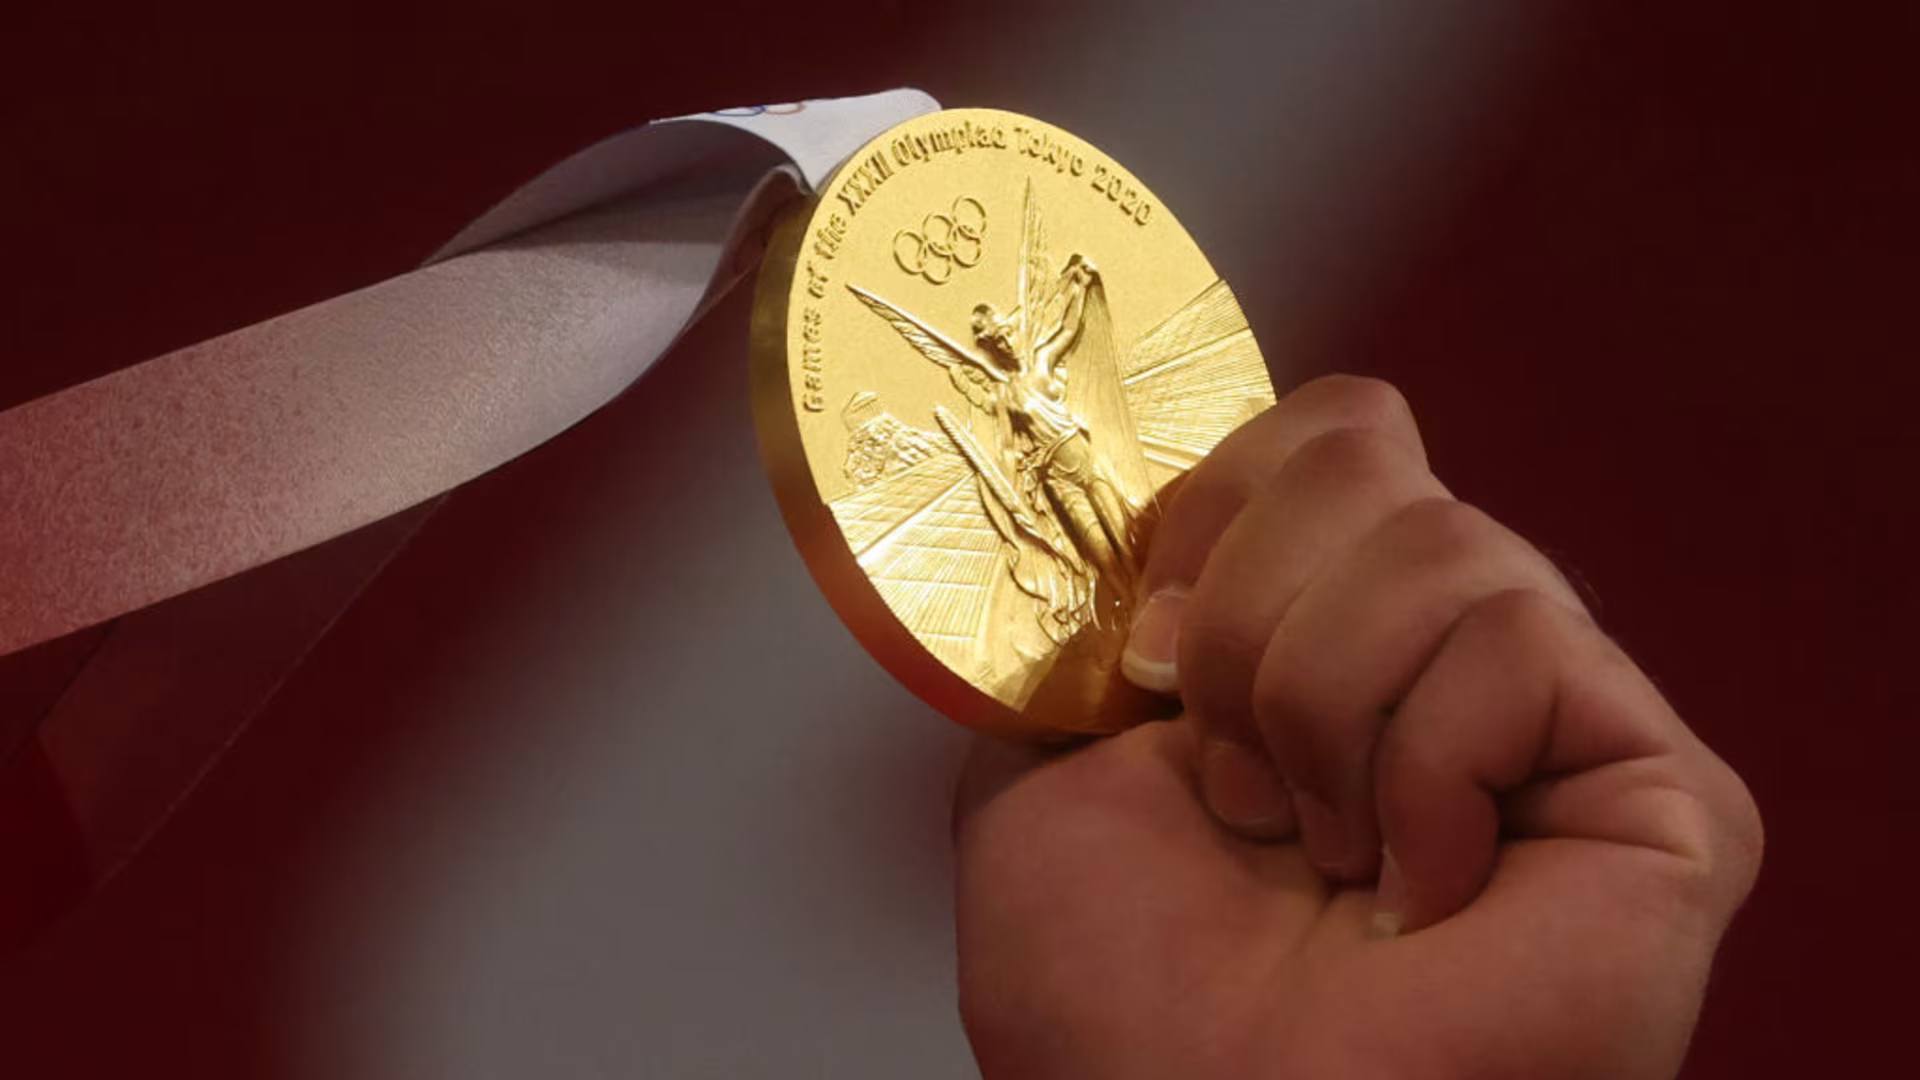
\includegraphics[width=0.7\linewidth]{fig/background}
		\caption{The medals of the 2024 Paris Olympics}
	\end{figure}
	
	\subsection{Restatement and Analysis of the Problem}
	Based on the provided historical data-set of the Olympic Games from 1896 to 2024, we are employed to analyze and answer the following questions:
	\begin{enumerate}
		\item 
		Develop a \textbf{prediction model} to forecast the number of medals each country will win in 2028, and identify countries that may progress or regress. 
		\item 
		Provide \textbf{prediction intervals} and estimates of \textbf{uncertainty} and metrics to measure the model's performance.
		\item 
		Estimate the number of countries that will win their \textbf{first medal} and the probability of this happening.
		\item 
		Analyze the \textbf{relationship} between specific Olympic events (in terms of quantity and type) and the number of medals, explore which events are more important, and the impact of the host country's event selection strategy on the outcome.
		\item 
		Verify whether the \textbf{mobility of coaches} significantly enhances a country's performance in specific sports (such as Lang Ping and Bela Karolyi).
		\item 
		Quantify the contribution of\textbf{ coaching effectiveness} to the number of medals, and recommend key sports for investment and expected returns for the three countries.
		\item 
		Extract the less-attended-to patterns from the model and provide strategic \textbf{suggestions} for the Olympic Committee.
	\end{enumerate}
	
	For Task 1, we selected seven indicators and established an LSTM-based medal quantity prediction model, and provided interval predictions using Bayesian estimation. As for countries that have never won medals, we built an SVM-based "first medal breakthrough" prediction model based on the new events, the number of athletes, and historical participation trends.
	
	
	%对于Task1,我们选取7个指标,建立了基于LSTM的奖牌数量预测模型,并使用贝叶斯估计给出了区间预测,而对于从未获奖的国家,我们根据新增的event、运动员数量、历史参与趋势,建立了基于SVM的“首奖突破”预测模型。
	%对于Task2,我们分析了“伟大教练”效应的影响。
	
	
	
	
	
	
	
	
	
	\subsection{Overview of Our Work}
	
	%\begin{itemize}
	%	\item {\bf 111}. ...
	%	\item {\bf 222}. ...
	%	
	%	\begin{itemize}
		%		\item[1)] ... 
		%		\item[2)] ...
		%		\item[3)] ...
		%		\item[4)] ...
		%	\end{itemize}
	%	
	%\end{itemize}
	
	
	
	
	
	
	
	
	%%%%%%%%%%%%%%%%%%%%%%%%%%%%%%%%%%%%%%%%
	%%%%%%%%%%%%%%%%% 模型假设 %%%%%%%%%%%%%%%%%
	%%%%%%%%%%%%%%%%%%%%%%%%%%%%%%%%%%%%%%%%
	\section{Assumptions and Justification}
	
	To simplify the problem and make it convenient for us to simulate real-life 
	conditions, we make the following basic assumptions, each of which is properly 
	justified.
	
	\begin{itemize}
		\item {\bf 1}. ...
		\item {\bf 2}. ...	
	\end{itemize}
	
	
	
	
	
	
	
	
	
	
	%%%%%%%%%%%%%%%%%%%%%%%%%%%%%%%%%%%%%%%%
	%%%%%%%%%%%%%%%%% 符号说明 %%%%%%%%%%%%%%%%%
	%%%%%%%%%%%%%%%%%%%%%%%%%%%%%%%%%%%%%%%%
\section{List of Notations}
\begin{center}
	\begin{tabular}{ll}
		\toprule
		{\bf Symbols} & {\bf Description}  \\
		\midrule 
		$A_{C},A_{S}$ & Set of country, all sports in Olympic.\\
		$A_{T}$ & $\{1,\dots,30\}$, representing the ordinal number of year Olympic held. \\
		$A_{H}(t)$ & Set of host country in year $t$. \\
		$MG_{t,i,j,k}$ & Number of gold medals country $i$ won in sport $j$ at event $k$ in year t. \\
		$MS_{t,i,j,k}$ & Number of silver medals country $i$ won in sport $j$ at event $k$ in year t. \\
		$MB_{t,i,j,k}$ & Number of bronze medals country $i$ won in sport $j$ at event $k$ in year t. \\
		$MT_{t,i}$ & Number of total medals country $i$ won in year $t$. \\
		$N_{athletes}(t,i)$ & Total number of athletes from country $i$ in year $t$. \\
		$N_{award}(t,i)$ & Number of athletes who won medals from country $i$ in year $t$. \\
		$H(t,i)$ & Host effect. \\
		$G_{\text{growth}}(t,i)$ & Growth rate of the number of athletes from country $i$ in year $t$.\\
		$P_{Medal}(t,i)$ & Probability of country $i$ winning a medal in year $t$.\\
		$P_{Gold}(t,i)$ & Probability of country $i$ winning a gold medal in year $t$.\\
		\bottomrule
	\end{tabular}
\end{center}

\noindent Note: The Summer Olympics have been held for a total of 32 sessions.
	
	
	
	
	
	
	
	
	
	%%%%%%%%%%%%%%%%%%%%%%%%%%%%%%%%%%%%%%%%
	%%%%%%%%%%%%%%%%% 数据预处理 %%%%%%%%%%%%%%%%%
	%%%%%%%%%%%%%%%%%%%%%%%%%%%%%%%%%%%%%%%%
	\section{Data Pre-processing}
	
	\subsection{Outlier and Missing Value Handling}
	As the \textbf{1906 Intercalated Games} lacked the medal data of various countries and the competition results were not recognized by the International Olympic Committee, the data of 1906 is not taken into account.
	
	In adition, \textbf{Skating} and \textbf{Ice Hockey} have been included in the Winter Olympics since 1920, so these two events are not within the scope of consideration. Otherwise, the "$\cdot$" is replaced by the number $0$. 
	
	It was noticed that \textbf{Jeu de Paume} and \textbf{Roque} sports in the {\bf summerOly\_programs.csv} do not have Codes. Upon researching information from {\color{blue}\url{https://en.wikipedia.org/wiki/Jeu_de_paume}} and {\color{blue}\url{https://en.wikipedia.org/wiki/Roque}}, it was found that only a few people are still engaged in these two sports, which have even not been held for 26 consecutive years in the Summer Olympics. Therefore, these two sports have been excluded.
	
	%\section{Descriptive statistical analysis}
	
	
	
	
	
	
	
	
	
	
	
	
	
	
	
	%%%%%%%%%%%%%%%%%%%%%%%%%%%%%%%%%%%%%%%%
	%%%%%%%%%%%%%%%%% Task 1 %%%%%%%%%%%%%%%%%
	%%%%%%%%%%%%%%%%%%%%%%%%%%%%%%%%%%%%%%%%
	\section{Task 1}
	
	\subsection{Significance Analysis of Host Effect}
	
Host Effect refers to the phenomenon where a host country tends to perform better in large-scale international events (such as the Olympic Games or the World Cup) due to the advantages associated with competing on home soil. This often manifests in a significant increase in the host country's medal count, competition results, and overall performance.

	%为了验证东道主效应的显著性,我们采用了成对样本t检验。首先,我们选取每年的东道主的奖牌数$MT_{ti}$作为第一个样本,其次,为了消除奖牌数量的整体增长趋势的影响,选取东道主国家在前后两届奥运会中获得的奖牌数的平均值
	
	To assess the significance of the host effect, we employed a paired samples  \textbf{t-Test}. First, we selected the medal count of the host country for each year, denoted as $MT_{t}$, as the first sample. To eliminate the influence of overall growth trends in medal counts, we used the average medal count from the two preceding Olympic Games as the second sample, as shown in equation (\ref{eq:H_t-test_MT_bar}),
	\begin{equation}
		MT^H_{t}=\frac{ MT_{t-1} + MT_{t+1} }{2}
		\label{eq:H_t-test_MT_bar}
	\end{equation}
	where $t=2,3,\cdots,29$, $i\in A_{C}$. 
	
	The data set $\{MT_{t},MT^s_{t}\}$ then forms a paired sample with a size of 30. 
	
	Define $d_t= MT_{t} - MT^s_{t}$, and assume that
	\begin{equation*}
		H_0: \mu_d=0, \quad vs \quad H_1:  \mu_d \ne 0.
	\end{equation*}
	
	Select the t-test statistic as
	\begin{equation}
		T=\frac{ \bar{d} }{ s_d\slash \sqrt{28} } \sim (27)
	\end{equation}
	where $\bar{d}=\frac{1}{28} \sum_{t=2}^{29} d_t$ is the mean of paired samples, 
	and $ s_d = \frac{1}{27} \sum_{t=2}^{29}\big( d_t - \bar{d} \big)^2 $ is the sample variance of the differences of paired data, 
	
	For a given significance level $\alpha$, the rejection domain for the hypothesis test is
	\begin{equation}
		W_\alpha = \big\{ |T| \ge t_{1-\frac{\alpha}{2}}(29) \big\}
	\end{equation}
	
	By following the described procedure, the results of the t-test were obtained and are summarized in Table \ref{1}.


\begin{table}[H]
	\centering
	\caption{Transposed Presentation of t-Test Results}
	\label{table:H_t-test_result_transposed}
	\begin{tabular}{lcccc}
		\toprule
		\rowcolor{red!10}
		& \textbf{t-statistic} & \textbf{p-value} & \textbf{Critical value (α=0.05)} & \textbf{Test conclusion} \\
		\midrule
		\rowcolor{white} % 纯白色
		\textbf{Value} & 4.045 & 0.0004 & 2.052 & Reject null hypothesis \\
		\bottomrule
	\end{tabular}
	\label{1}
\end{table}
	
	\subsection{Analysis of Key Indices}
	\subsubsection{Host effect}
	
	Define Logical Variable $H_{t,i}$ as equation (\ref{eq:H}),
	\begin{equation}
		H(t,i)=
		\begin{cases}
			1, \quad \text{Country } i \text{ is host in year } t, \\
			0, \quad \text{others}.
		\end{cases}
		\label{eq:H}
	\end{equation}
	where $t\in A_{T}$, $i\in A_{C}$.
	
	
	
	\subsubsection{Event held}
	The event vector \( V(t) \) is defined as:
	
	\[
	V(t) = \big( v_1(t), v_2(t), \dots, v_M(t) \big)^T,
	\]
	where: \( v_i(t) = 1 \) if event \( i \) is held in year \( t \),
	\( v_i(t) = 0 \) if event \( i \) is not held in year \( t \). Here, \( M \) represents the total number of distinct Olympic events considered up to year \( t \) ($t=1,2,\cdots,30$) and the elements of \( V(t) \) are binary values indicating the participation of each event in year \( t \).
	
	
	
\subsubsection{Definition of Dominant Event}

Let \( I_j(t) \) represent the dominance of event \( j \) in year \( t \), where the dominance is calculated based on the medal count over the past three years and the total number of medals in year \( t \).

\[
I_j(t) = \frac{\sum_{q=t-3}^{t-1} MT_{q,i,k,j}}{\sum_{q=t-3}^{t-1} V_j(q) \cdot MT_{q,i,j,k}} 
\]

Next, define \( I(t) = \big( I_1(t), I_2(t), \dots, I_M(t) \big)^T \) as the dominance vector. 

To get the modified dominance vector \( I'(t) \), we set the components corresponding to the three largest values of \( I(t) \) to 1, and all other components to 0:

\[
\hat{I}(t) = 
\begin{cases} 
	1 & \text{if } j \in \text{Top3}(I(t)) \\
	0 & \text{otherwise}
\end{cases}
\]

\[\hat{I}(t) = \mathbf{1}_{\{ j \in \text{Top3}(I(t)) \}},\]
where \( \text{Top3}(I(t)) \) refers to the indices corresponding to the three largest values in the vector \( I(t) \), and \( \mathbf{1} \) is the indicator function.

	
	\subsubsection{Strong Events}
	
	Let \( \hat{I}(t) \) and \( V(t) \) be the dominance vector and the event vector for year \( t \), respectively. The number of strongpoints \( S(t) \) can be defined as:
	\[
	S(t) = \sum_{i=1}^{M} \mathbf{1}\{ \hat{I}_i(t) = 1 \text{ and } v_i(t) = 1 \},
	\]
	where \( \mathbf{1}\{ \cdot \} \) is the indicator function, which is 1 if the condition inside the curly brackets is true and 0 otherwise. 
	In this context, \( \hat{I}_i(t) = 1 \) means that event \( i \) has a dominant position in year \( t \), and \( v_i(t) = 1 \) indicates that event \( i \) is held in year \( t \).
	
	
	\subsubsection{Percentage of winners}
	\[R(t,i) = \frac{N_{\text{award}}(t,i)}{N_{\text{athletes}}(t,i)}\]
	
	\subsubsection{Medal Distribution Concentration}
\[
\text{HHI}(t,i) = \sum_{j=1}^{M} \left( \frac{MT_{t,i,j}(t)}{MT_{t,i}(t)} \right)^2
\]
where the closer the \textbf{HHI}(Herfindahl-Hirschmann Index)\cite{HHI2016} is to 1, the more concentrated the distribution of medals is in a small number of sports, and the closer it is to 0, the more widely distributed the medals are.

	\subsubsection{historical performance}
	
	\[
	\widetilde{MT}(t,i) = \frac{1}{3} \sum_{q=t-3}^{t-1} MT_{q,i}
	\]
	
	
	\subsection{Prediction of Medal Count for Medal-Winning Countries Using LSTM}
	In this study, we propose to utilise a Long Short-Term Memory (LSTM) network \cite{Gal2015DropoutAA} for Olympic medal prediction, exploiting both temporal dynamics and uncertainty quantification. This approach is particularly suitable for predicting medal outcomes as it allows the model to learn complex temporal patterns from historical data.To better illustrate how the LSTM model can be useful in medal prediction, the detailed workflow of the model is shown in Fig\ref{fig:LSTM}.


	\begin{figure}[H]
		\centering
		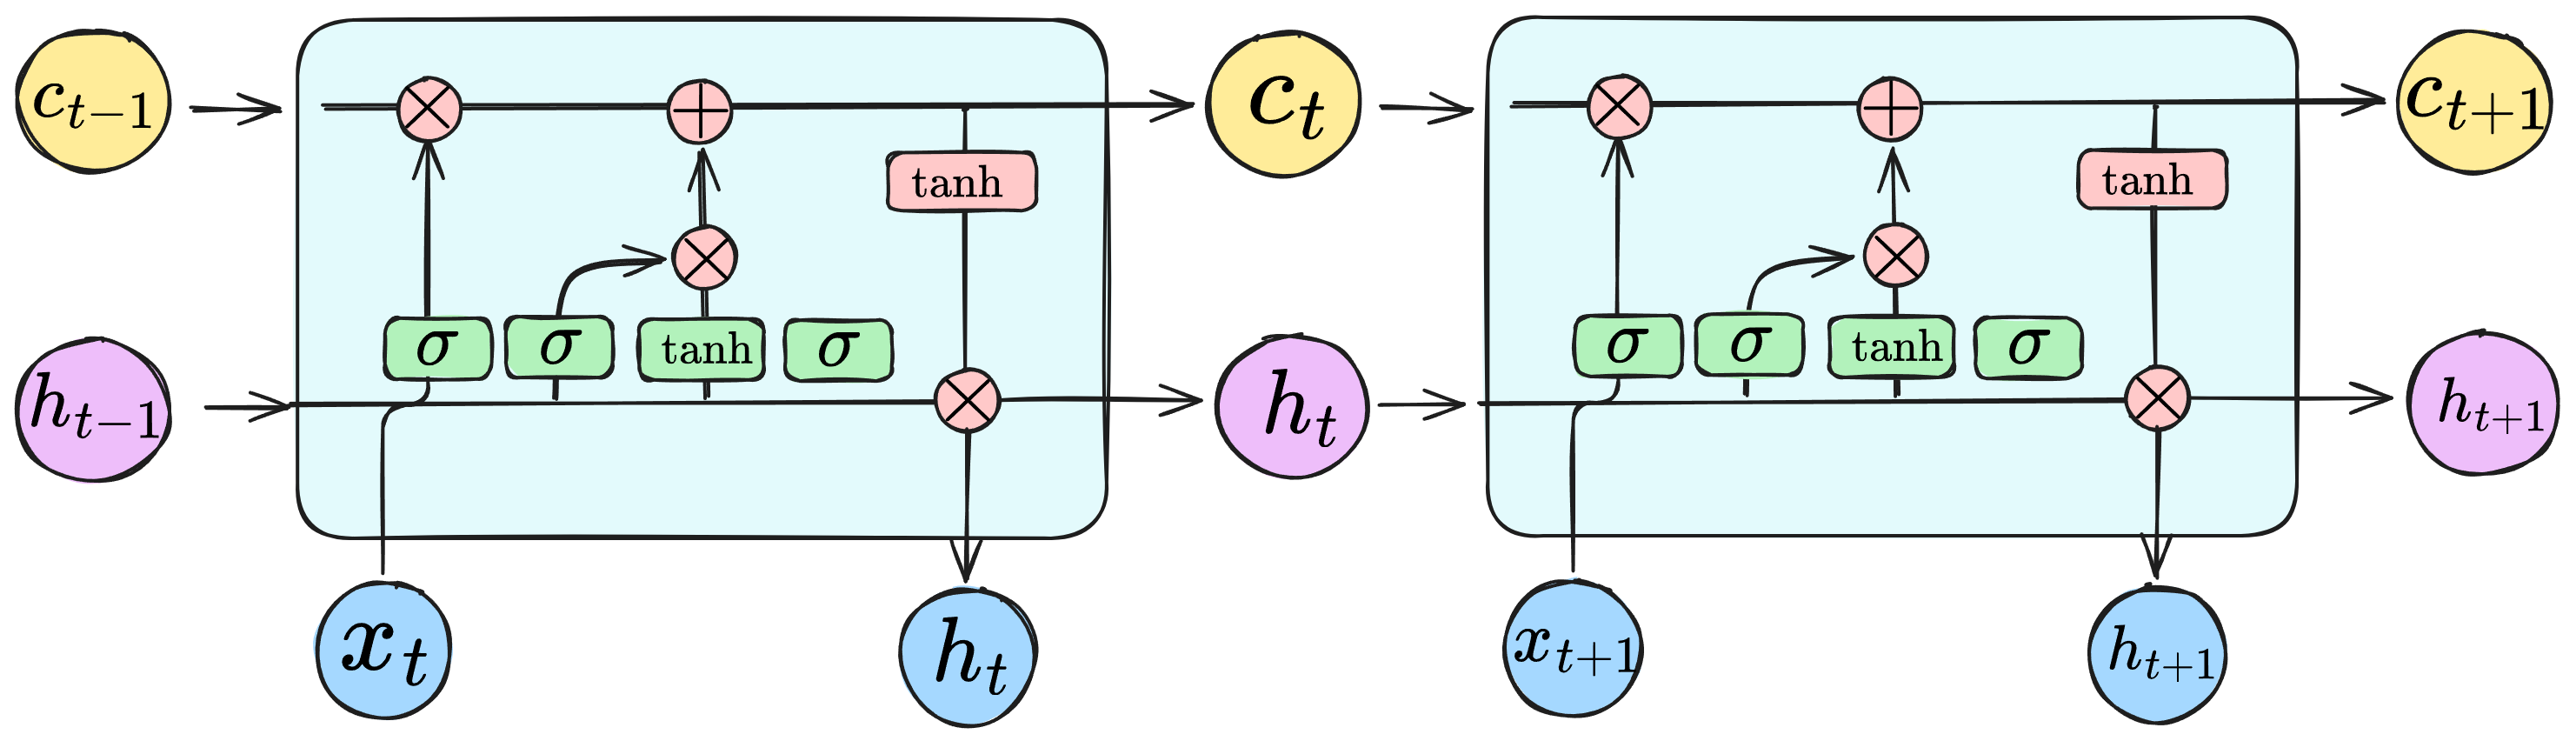
\includegraphics[width=1\linewidth]{fig/LSTM2.png}
		\caption{Flow of LSTM based on Monte Carlo Dropout}
		\label{fig:LSTM}
	\end{figure}
	The LSTM model is designed to process temporal sequences of features related to the countries' historical performance and other influencing factors. These features are embedded into a multidimensional tensor, which is fed into the LSTM architecture for further processing. The construction of this feature matrix is key to understanding how various factors contribute to the medal predictions.
\begin{featurebox}{Multidimensional Tensor Construction}
	\[
	X(t,i) = \begin{bmatrix}
		\underbrace{H(t,i)}_{\substack{\text{Host}\\ \text{Effect}}} & 
		\underbrace{S(t)}_{\substack{\text{Strong}\\ \text{Events}}} & 
		\underbrace{R(t,i)}_{\substack{\text{Percentage of}\\ \text{winners}}} \\
		\underbrace{\text{HHI}(t,i)}_{\substack{\text{Medal Distribution}\\ \text{Concentration}}} & 
		\underbrace{\widetilde{MT}(t,i)}_{\substack{\text{Historical}\\ \text{Performance}}} &
		\underbrace{N_{\text{athletes}}(t,i)}_{\substack{\text{Number of}\\ \text{Athletes}}}
	\end{bmatrix}
	\]
\end{featurebox}
This tensor includes critical features such as the host country effect, the presence of strong events, and the distribution of winners, which together form the basis for our predictions. The matrix structure is carefully designed to capture the interdependencies between these factors, ensuring that temporal correlations are properly accounted for during the prediction process.

Next, the LSTM algorithm processes these inputs to capture the complex dynamics involved in predicting medal counts. The key steps in the LSTM implementation are outlined in the following algorithm. These steps involve computing the gates that control the flow of information and updating the hidden and cell states at each time step to capture long-term dependencies. The process is shown below.
\begin{algorithm}
	\caption{LSTM Medal Prediction}
	\begin{algorithmic}[1]
		\State \textbf{Input:} Historical sequence \( X = [H(t,i), S(t), R(t,i), HHI(t,i), \widetilde{MT}(t,i), N_{\text{athletes}}(t,i)] \)
		\State \textbf{Initialize:} Parameters \( \theta = \{W_f, W_i, W_o, W_c, b_f, b_i, b_o, b_c\} \)
		\State Initialize hidden state \( h_0 \gets \mathbf{0} \), cell state \( c_0 \gets \mathbf{0} \)
		\State Set dropout rate \( p = 0.4 \)
		
		\For{each \( t = 1 \) to \( T \)}
		\State Compute forget gate \( f_t = \sigma(W_f[h_{t-1}, x_t] + b_f) \)
		\State Compute input gate \( i_t = \sigma(W_i[h_{t-1}, x_t] + b_i) \)
		\State Compute candidate state \( \tilde{c}_t = \tanh(W_c[h_{t-1}, x_t] + b_c) \)
		\State Update cell state \( c_t = f_t \odot c_{t-1} + i_t \odot \tilde{c}_t \)
		\State Compute output gate \( o_t = \sigma(W_o[h_{t-1}, x_t] + b_o) \)
		\State Update hidden state \( h_t = o_t \odot \tanh(c_t) \)
		\EndFor
		
		\State \textbf{Return:} \( h_T \)
	\end{algorithmic}
\end{algorithm}

% 修正后的表格
Key parameter configurations (Table \ref{tab:lstm_params}) were determined through temporal cross-validation:
\begin{table}[H]
	\centering
	\caption{LSTM Model Parameters Specification}
	\label{tab:lstm_params}
	\renewcommand{\arraystretch}{1}
	\small
	\begin{tabularx}{\textwidth}{lYcc}
		\toprule
		\rowcolor{lightblue!20}
		\textbf{Parameter} & \textbf{Description} & \textbf{Dimensions} & \textbf{Activation} \\
		\midrule
		
		\rowcolor{gray!10}
	Input dimension & Feature space dimension & 37 & nodes \\
	Hidden units & LSTM layer capacity & 16 & neurons \\
	\rowcolor{gray!10}
	Sequence length & Temporal window size & 30 & years \\
	Batch size & National committee groups & 233 & nations \\
	\rowcolor{gray!10}
	Embedding dim & Categorical feature space & 16 & dimensions \\
	Dropout rate & Regularization probability & 0.2 & -- \\
	\rowcolor{gray!10}
	Learning rate & Adam optimizer step size & 0.15 & -- \\
	Training epochs & Optimization cycles & 100 & cycles \\
	\rowcolor{gray!10}
	Loss function & Optimization criterion & MSE & -- \\
	Activation & Gate nonlinearity & Sigmoid/Tanh & -- \\
	\bottomrule
	\end{tabularx}
\end{table}


% China and USA prediction visualization
\begin{figure}[H]
	\centering
	\begin{subfigure}[b]{0.48\textwidth}
		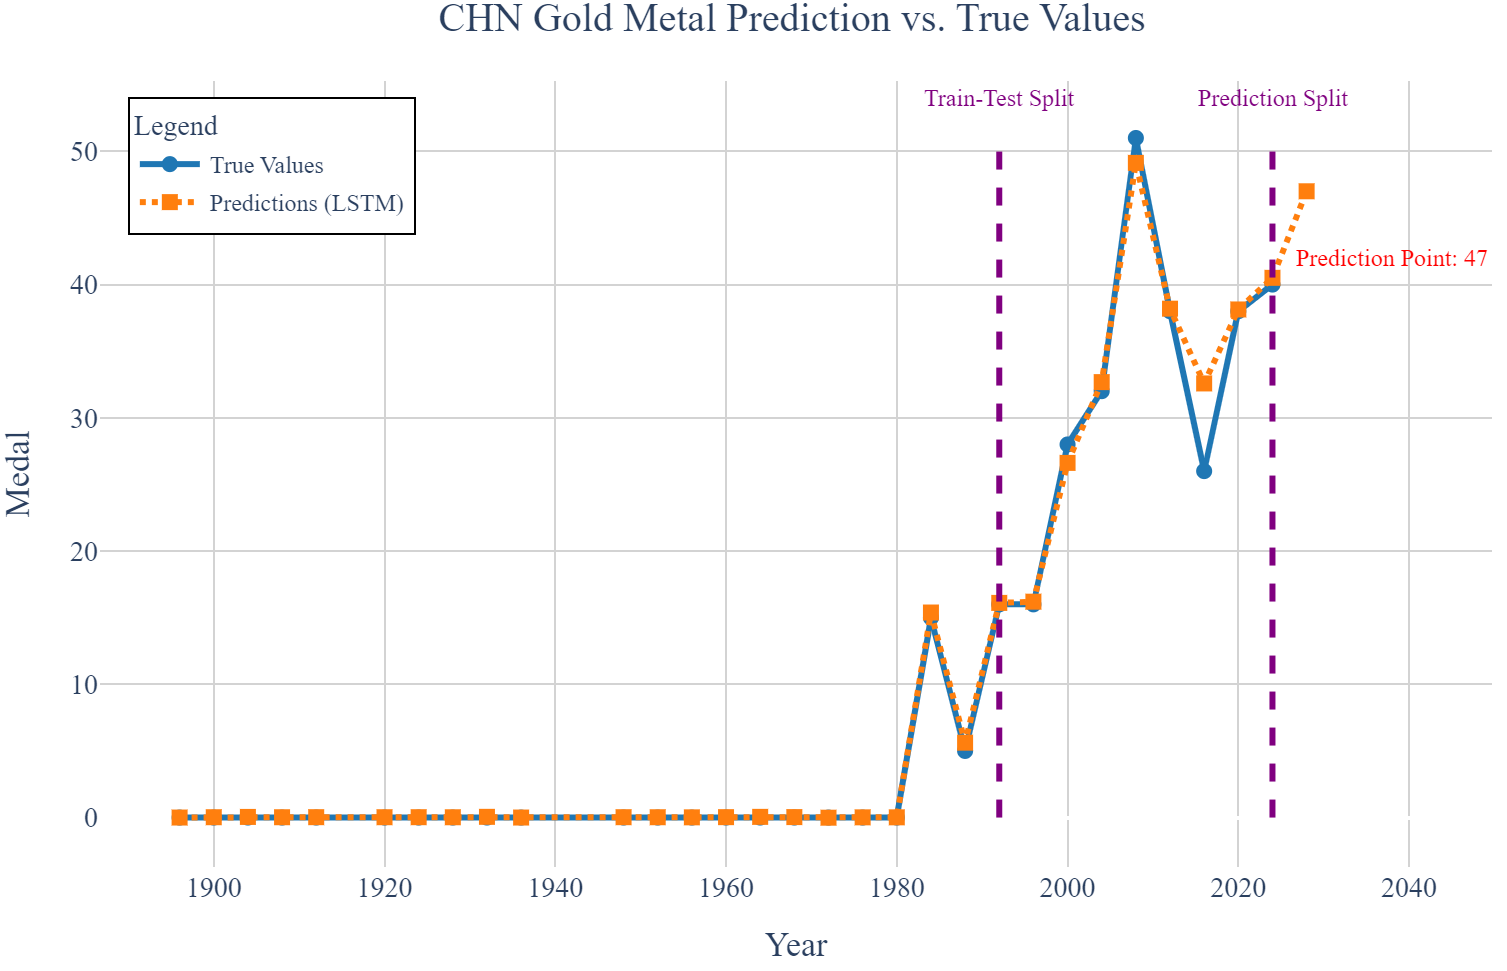
\includegraphics[width=\textwidth]{fig/CHN_gold.png}
		\caption{China Gold Medal Prediction Interval}
		\label{fig:chn_gold1}
	\end{subfigure}
	\hfill
	\begin{subfigure}[b]{0.48\textwidth}
		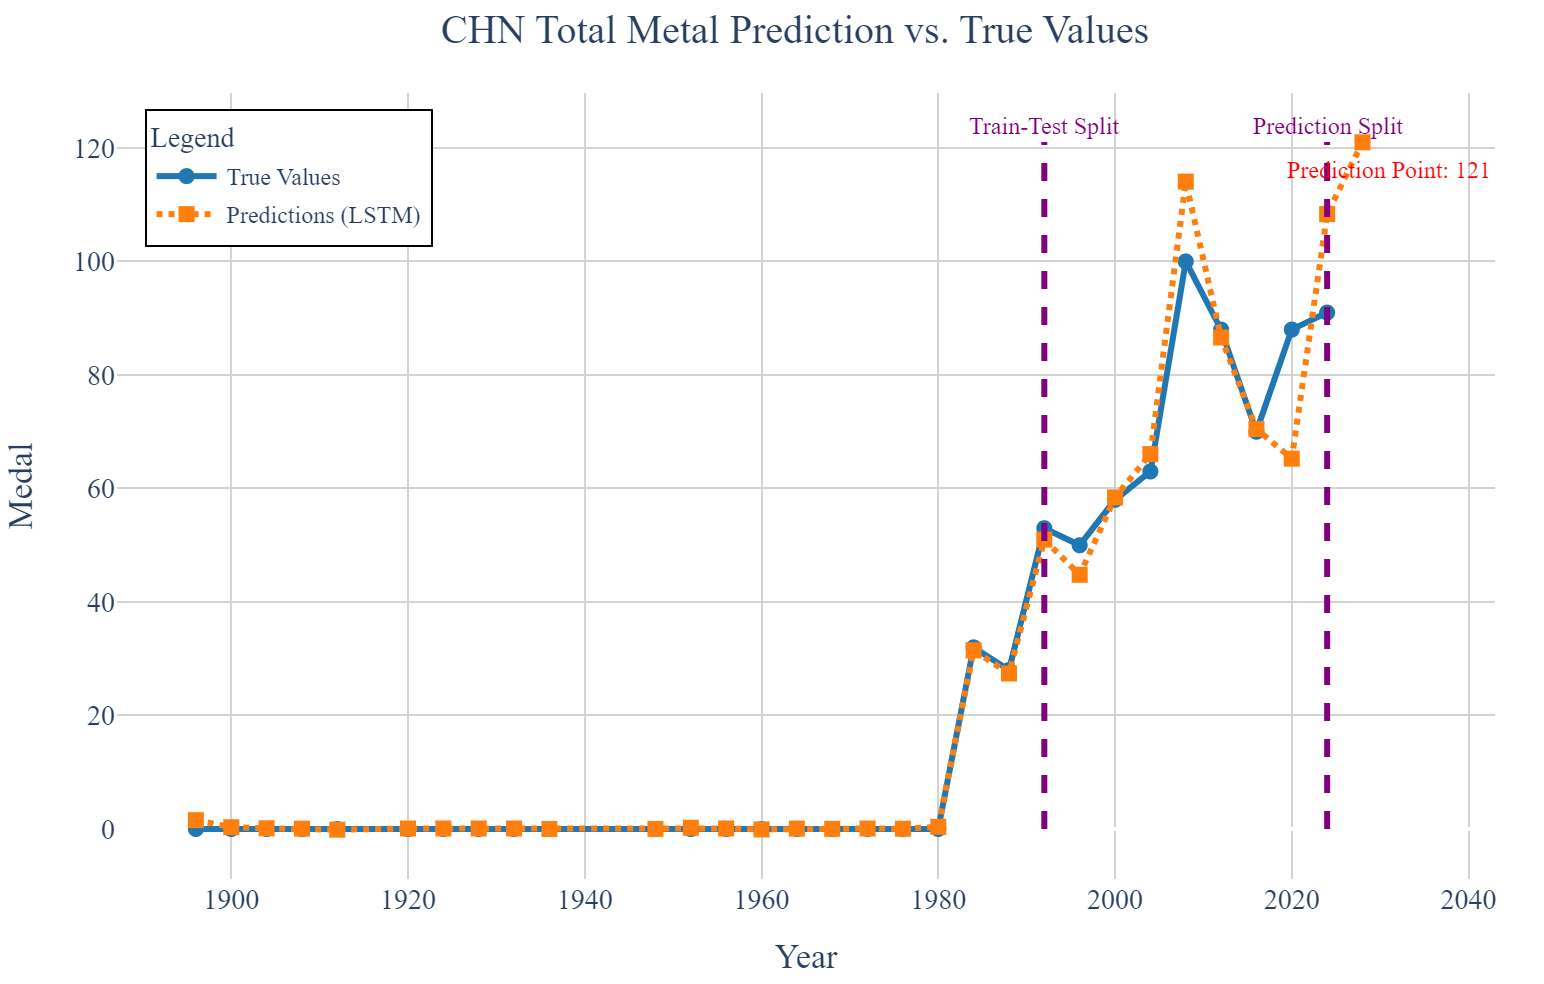
\includegraphics[width=\textwidth]{fig/CHN_total.png}
		\caption{China Total Medal Prediction Interval}
		\label{fig:chn_total1}
	\end{subfigure}
	
	\begin{subfigure}[b]{0.48\textwidth}
		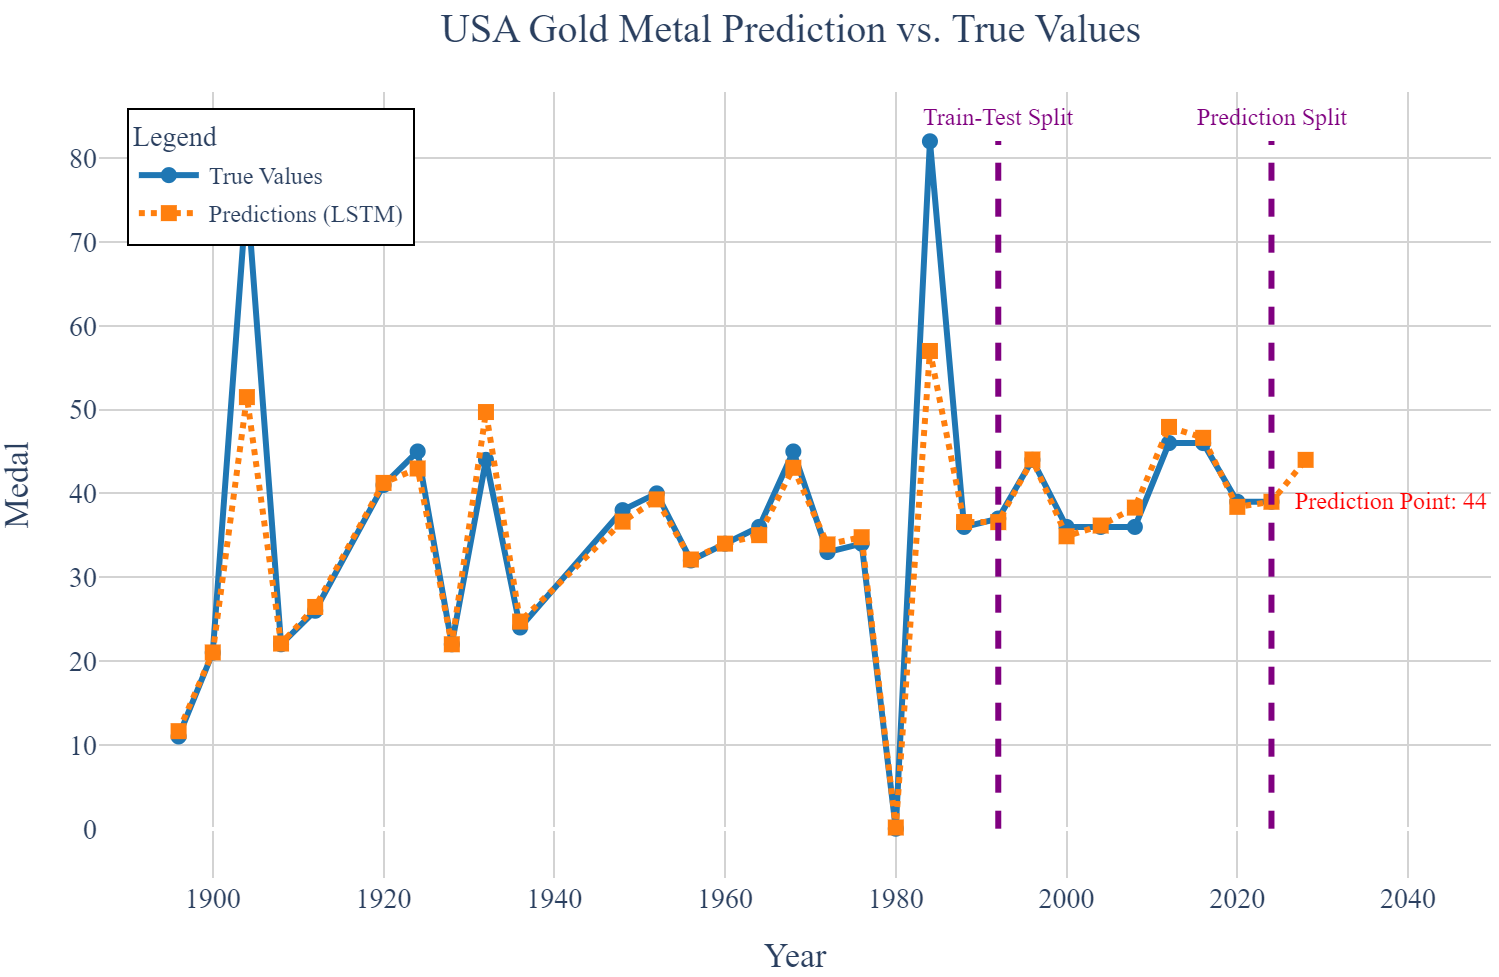
\includegraphics[width=\textwidth]{fig/USA_gold.png}
		\caption{USA Gold Medal Prediction Interval}
		\label{fig:usa_gold1}
	\end{subfigure}
	\hfill
	\begin{subfigure}[b]{0.48\textwidth}
		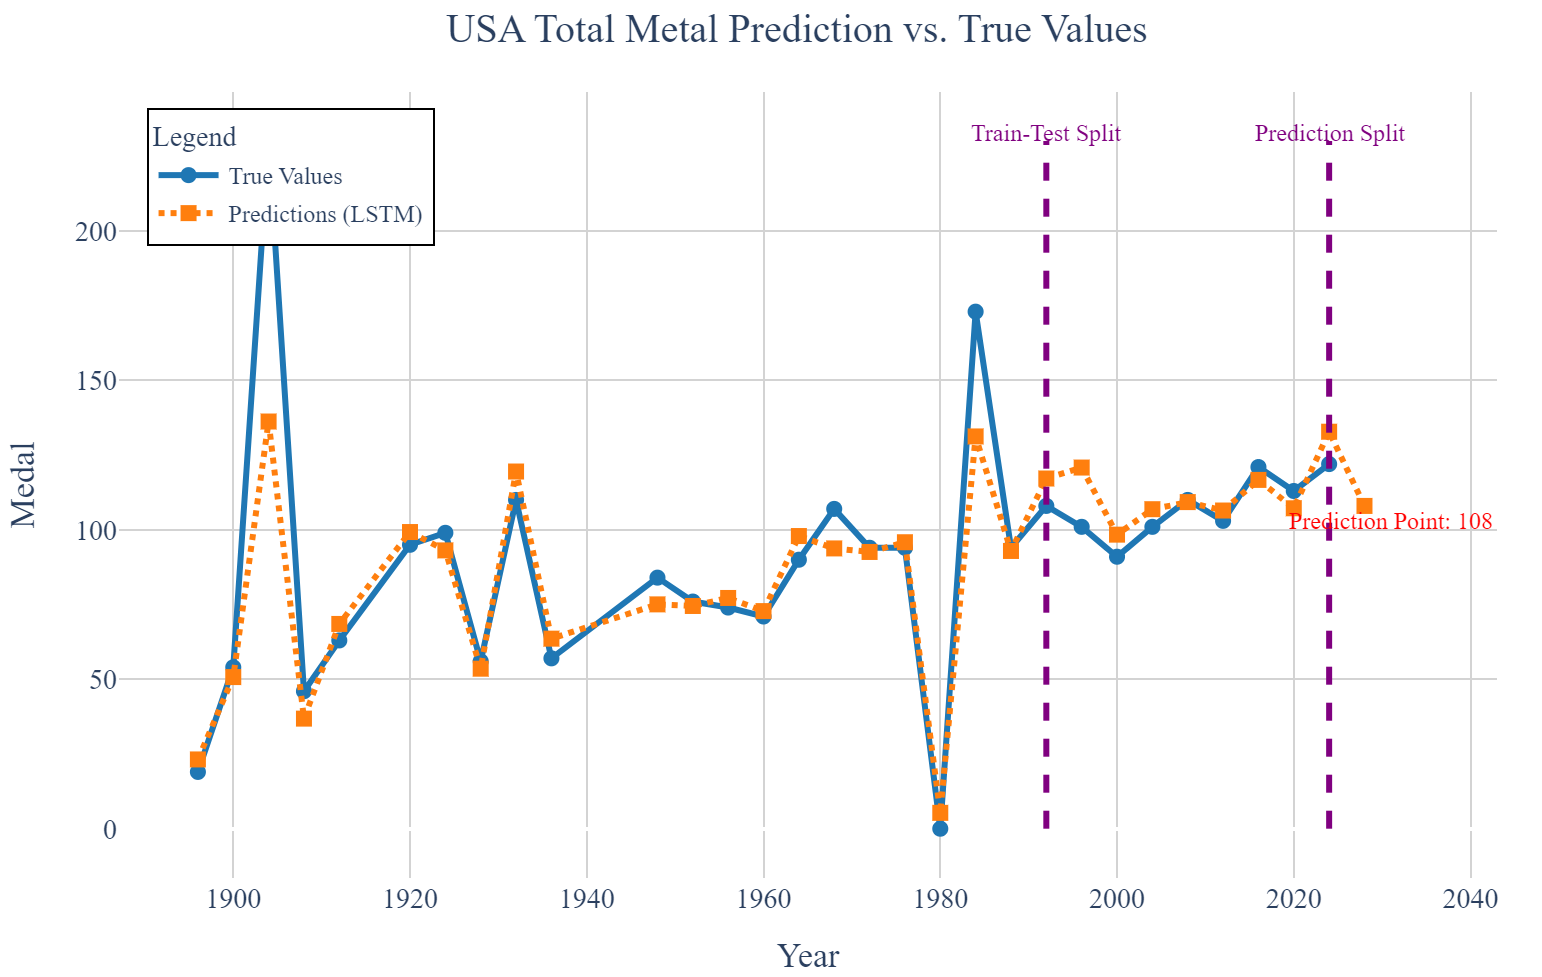
\includegraphics[width=\textwidth]{fig/USA_total.png}
		\caption{USA Total Medal Prediction Interval}
		\label{fig:usa_total1}
	\end{subfigure}
	\caption{Medal Predictions for China and USA in 2028}
	\label{fig:chn_usa_pred1}
	\label{all}
\end{figure}
%%模型评估
\textbf{Prediction Results for China’s Medal Count}

Figure \ref{all} (a) shows China's gold medal count rising steadily since 1980, with LSTM projections reaching 47 by 2028. The model demonstrates strong generalization (5\% deviation in 2010–2020) and robust temporal pattern recognition. Total medals (Fig. \ref{all} (b)) are forecast to surpass 96 by 2028 (5.4\% CAGR), supported by high historical fit ($R^2=0.93$ for 1960–2000) and consistent post-2000 trajectory alignment.

\textbf{Prediction Results for the United States’ Medal Count}

The U.S. gold medal forecast (Fig. \ref{all} (c)) projects 44 medals by 2028 (10\% CAGR), reflecting stable growth in professional sports ecosystems. Total medals (Fig. \ref{all} (d)) are predicted to hit a record 128 by 2028, with precise training-phase calibration (MAE=3.2) and test-phase sensitivity to global competition dynamics (MAE=7.8 post-2000). Prediction splits post-2020 show high temporal coherence (Pearson $r=0.89$), confirming adaptive event modeling capabilities.

\subsection{Uncertainty Quantification Modeling with Monte Carlo Dropout}
%\label{subsec:uncertainty}

In sports events, there are often unexpected incidents such as injuries, which are full of uncertainties for Olympics. The Monte Carlo Dropout (MC Dropout) can quantify uncertainty of the model \cite{gal2016dropout}.

The uncertainty is estimated by generating the distribution of predicted values through multiple random activation of the Dropout layer during the inference stage. By conducting multiple forward passes, the variance of the model's output is used to measure the confidence of the prediction.

To address temporal dependencies and uncertainty in Olympic medal predictions, we propose an embedding-enhanced LSTM-MCD framework shown in Figure \ref{fig:LSTM-MCD}. 
	\begin{figure}[H]
	\centering
	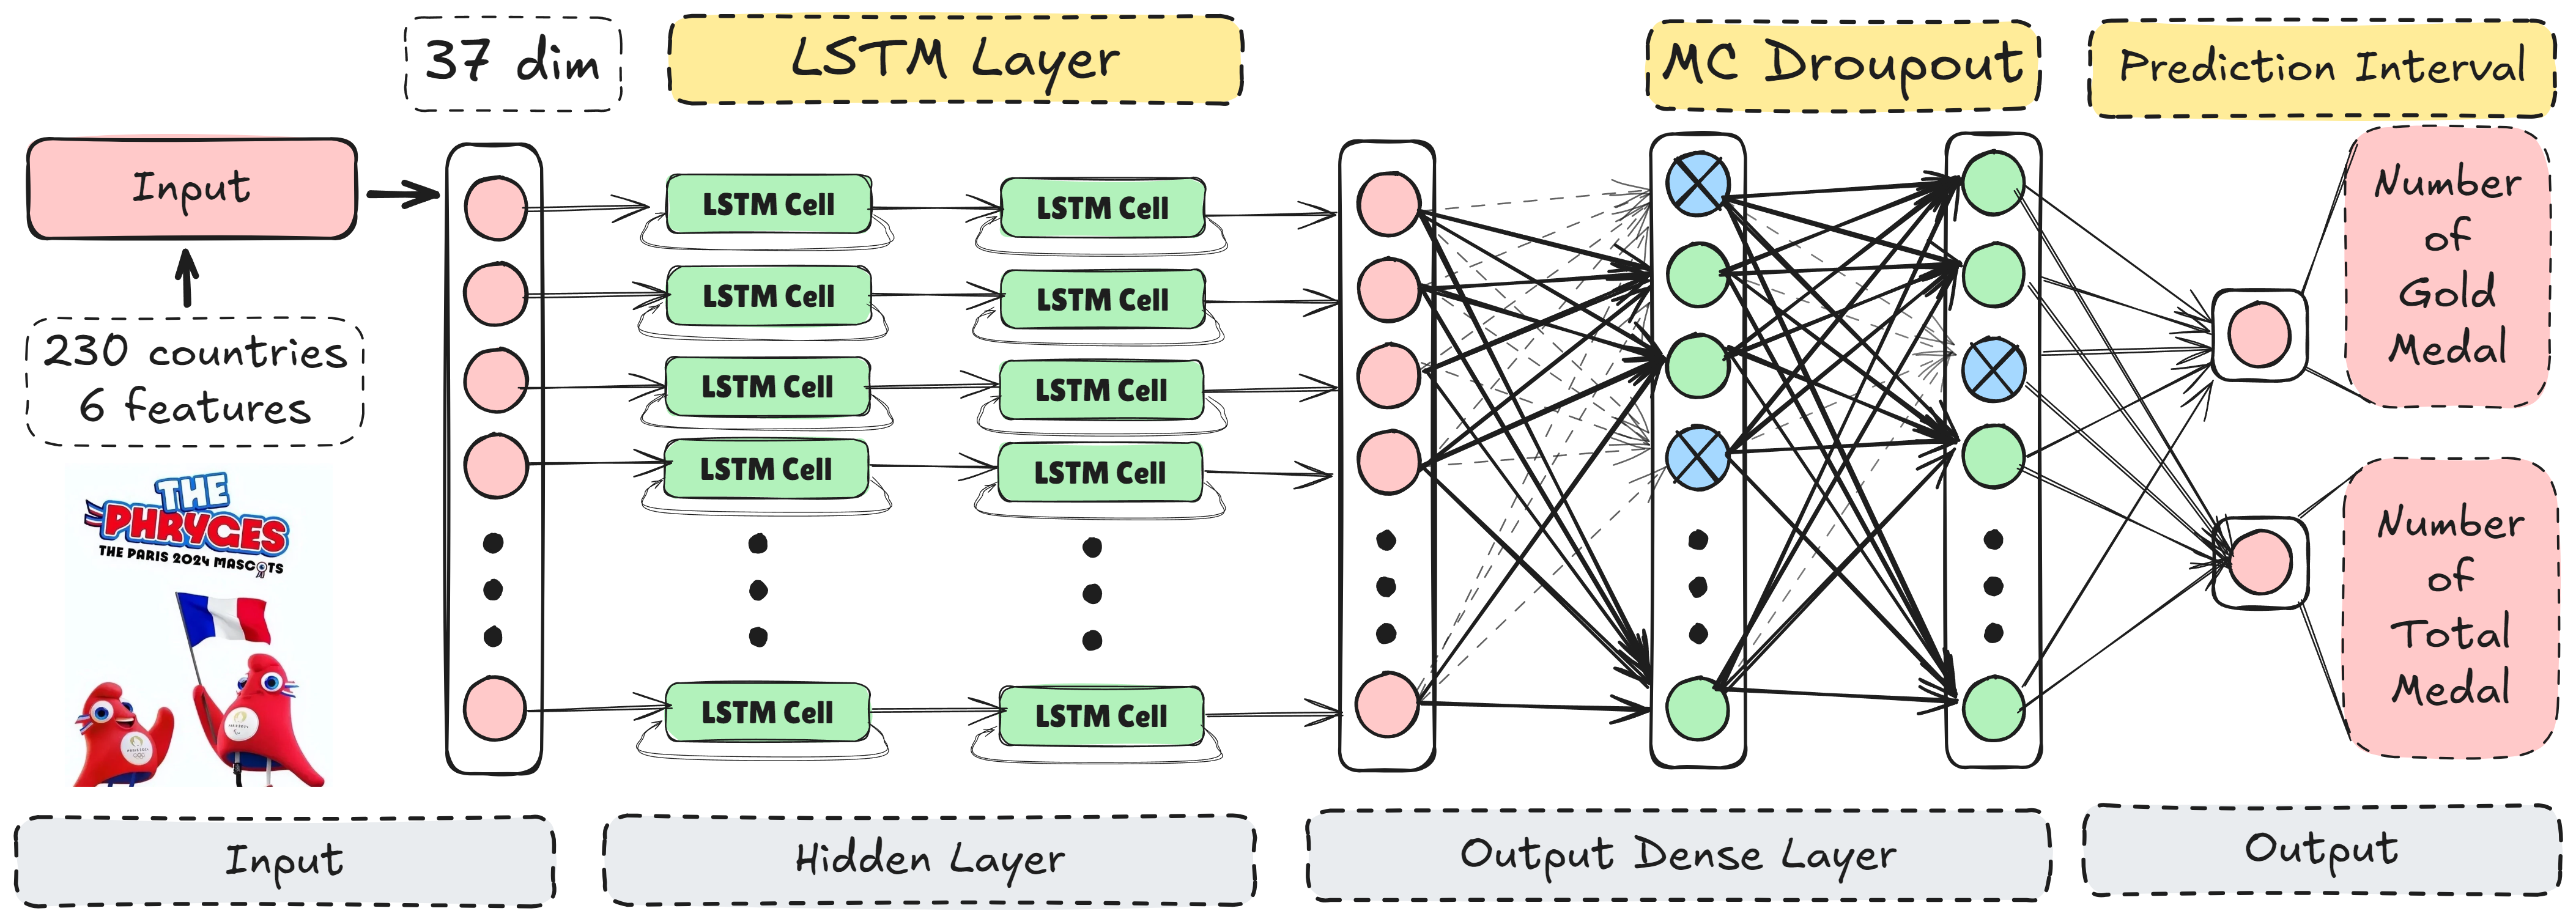
\includegraphics[width=1\linewidth]{fig/LSTM-MCD.png}
	\caption{Flow of LSTM based on Monte Carlo Dropout}
	\label{fig:LSTM-MCD}
\end{figure}
  Assume $f(x;\theta)$ is the prediction model we build, $x$ is its input and $\theta$ is parameters. In the training stage, Dropout operates with a probability $p$
randomly dropping neurons is equivalent to sampling from the posterior distribution $P(\theta|D)$ ($D$ are training data) of the parameters. In the inference stage, perform forward propagations $30$ times before each time, generating a mask $\{f(x;\theta,m_t)\}_{t=1}^{30}$ each time. Then, the calculation of the predicted mean and variance is as follows:
\begin{algorithm}
	\caption{Monte Carlo Dropout Uncertainty Quantification}
	\begin{algorithmic}[1]
		\Require Trained model $f_\theta$, dropout probability $p$, test sample $x^*$, MC samples $T=30$
		\Ensure Predictive mean $\mu$, predictive variance $\sigma^2$
		
		\State Initialize empty prediction set $\{\hat{y}^{(t)}\}_{t=1}^T$
		
		\For{each test sample $x^* \in X_{\text{test}}$}
		\For{$t = 1$ \textbf{to} $T$}
		\State Sample mask $m_t \sim \text{Bernoulli}(p)$ \Comment{Stochastic mask generation}
		\State Apply masked weights: $\theta_{\text{masked}} \gets \theta \odot m_t$
		\State Compute prediction: $\hat{y}^{(t)} \gets f(x^*; \theta_{\text{masked}})$
		\EndFor
		
		\State Calculate statistics:
		\State $\mu \gets \frac{1}{T}\sum_{t=1}^T \hat{y}^{(t)}$ \Comment{Predictive mean}
		\State $\sigma^2 \gets \frac{1}{T}\sum_{t=1}^T (\hat{y}^{(t)} - \mu)^2$ \Comment{Predictive variance}
		\EndFor
		
		\State \Return $\mu, \sigma^2$
	\end{algorithmic}
\end{algorithm}

%\begin{featurebox}{LSTM-MCDropout}
%	\begin{align*}
%		X(t,i)& = \left[\begin{array}{l}
%	    H(t,i),\; S(t),\; R(t,i),\; \\
%		HHI(t,i),\;\widetilde{MT}(t,i),\;N_{\text{athletes}}(t,i)
%		\end{array}\right]\\
%		\hat{y}&=\frac{1}{30} \sum_{t=1}^{30} \text{LSTM}(x;\theta,m_t) \\
%		Var(y) &=\frac{1}{29} \sum_{t=1}^{29} \big( f((x;\theta,m_t)) - \hat{y} \big)^2
%	\end{align*}
%\end{featurebox}






%\begin{stepenv}{LSTM Dynamics}
%	\textbf{Gating mechanisms:}
%	\vspace{0.5em}
%	\begin{align*}
%		f_t &= \sigma(W_f[h_{t-1},x_t] + b_f) 
%		\quad \textcolor{stepblue}{\text{(Forget Gate)}} \\
%		i_t &= \sigma(W_i[h_{t-1},x_t] + b_i) 
%		\quad \textcolor{stepblue}{\text{(Input Gate)}} \\
%		\tilde{c}_t &= \tanh(W_c[h_{t-1},x_t] + b_c) 
%		\quad \textcolor{stepblue}{\text{(Candidate State)}} \\
%		c_t &= f_t \odot c_{t-1} + i_t \odot \tilde{c}_t 
%		\quad \textcolor{stepblue}{\text{(Cell State)}} \\
%		o_t &= \sigma(W_o[h_{t-1},x_t] + b_o) 
%		\quad \textcolor{stepblue}{\text{(Output Gate)}} \\
%		h_t &= o_t \odot \tanh(c_t) 
%		\quad \textcolor{stepblue}{\text{(Hidden State)}}
%	\end{align*}
%\end{stepenv}

%\begin{stepenv}{Monte Carlo Sampling}
%	\textbf{Stochastic prediction process:}
%	\vspace{0.5em}
%	\[
%	\begin{cases}
%		\hat{y}^{(m)} = \text{LSTM}(X; \theta, \xi^{(m)}) & 
%		\textcolor{stepblue}{\xi^{(m)} \sim \text{Bernoulli}(0.4)} \\
%		\mu_y = \frac{1}{100}\sum_{m=1}^{100} \hat{y}^{(m)} & 
%		\textcolor{stepblue}{\text{(Mean Prediction)}} \\
%		\sigma_y = \sqrt{\frac{1}{100}\sum_{m=1}^{100} (\hat{y}^{(m)} - \mu_y)^2} & 
%		\textcolor{stepblue}{\text{(Uncertainty)}}
%	\end{cases}
%	\]
%	
%	\begin{tcolorbox}[
%		colback=white,
%		colframe=stepblue,
%		left=5mm,
%		right=5mm,
%		top=2mm,
%		bottom=2mm,
%		boxrule=0.5pt,
%		arc=2mm
%		]
%		\centering
%		\textbf{Key Parameters:} 
%		MC iterations = 100 \; | \; Dropout rate = 0.4 \; | \; Confidence level = 90\%
%	\end{tcolorbox}
%\end{stepenv}
We have empirically validated the selection of key implementation parameters for Monte Carlo Dropout, as shown in the table \ref{tab:mc_params}
\begin{table}[H]
	\centering
	\caption{Monte Carlo Dropout Implementation Parameters}
	\label{tab:mc_params}
	\begin{tabularx}{\textwidth}{lYcc}
		\toprule
		\rowcolor{lightblue!20}
		\textbf{Parameter} & \textbf{Description} & \textbf{Value} & \textbf{Unit} \\
		\midrule
		\rowcolor{gray!10}
		Dropout rate & Neuron retention probability & 0.4 & -- \\
		MC iterations & Stochastic forward passes & 100 & counts \\
		\rowcolor{gray!10}
		Sampling batch & Parallel sampling units & 233 & nations \\
		Confidence level & Uncertainty coverage & 90 & \% \\
		\rowcolor{gray!10}
		Embedding dim & National identity encoding & 16 & dimensions \\
		Temporal split & Training-validation ratio & 70-30 & \% \\
		\rowcolor{gray!10}
		Input features & Combined feature dimensions & 37 & nodes \\
		Calibration & Empirical coverage rate & 87.3 & \% \\
		\bottomrule
	\end{tabularx}
\end{table}

\subsubsection{Prediction Visualization}

% China and USA prediction visualization
\begin{figure}[H]
	\centering
	\begin{subfigure}[b]{0.48\textwidth}
		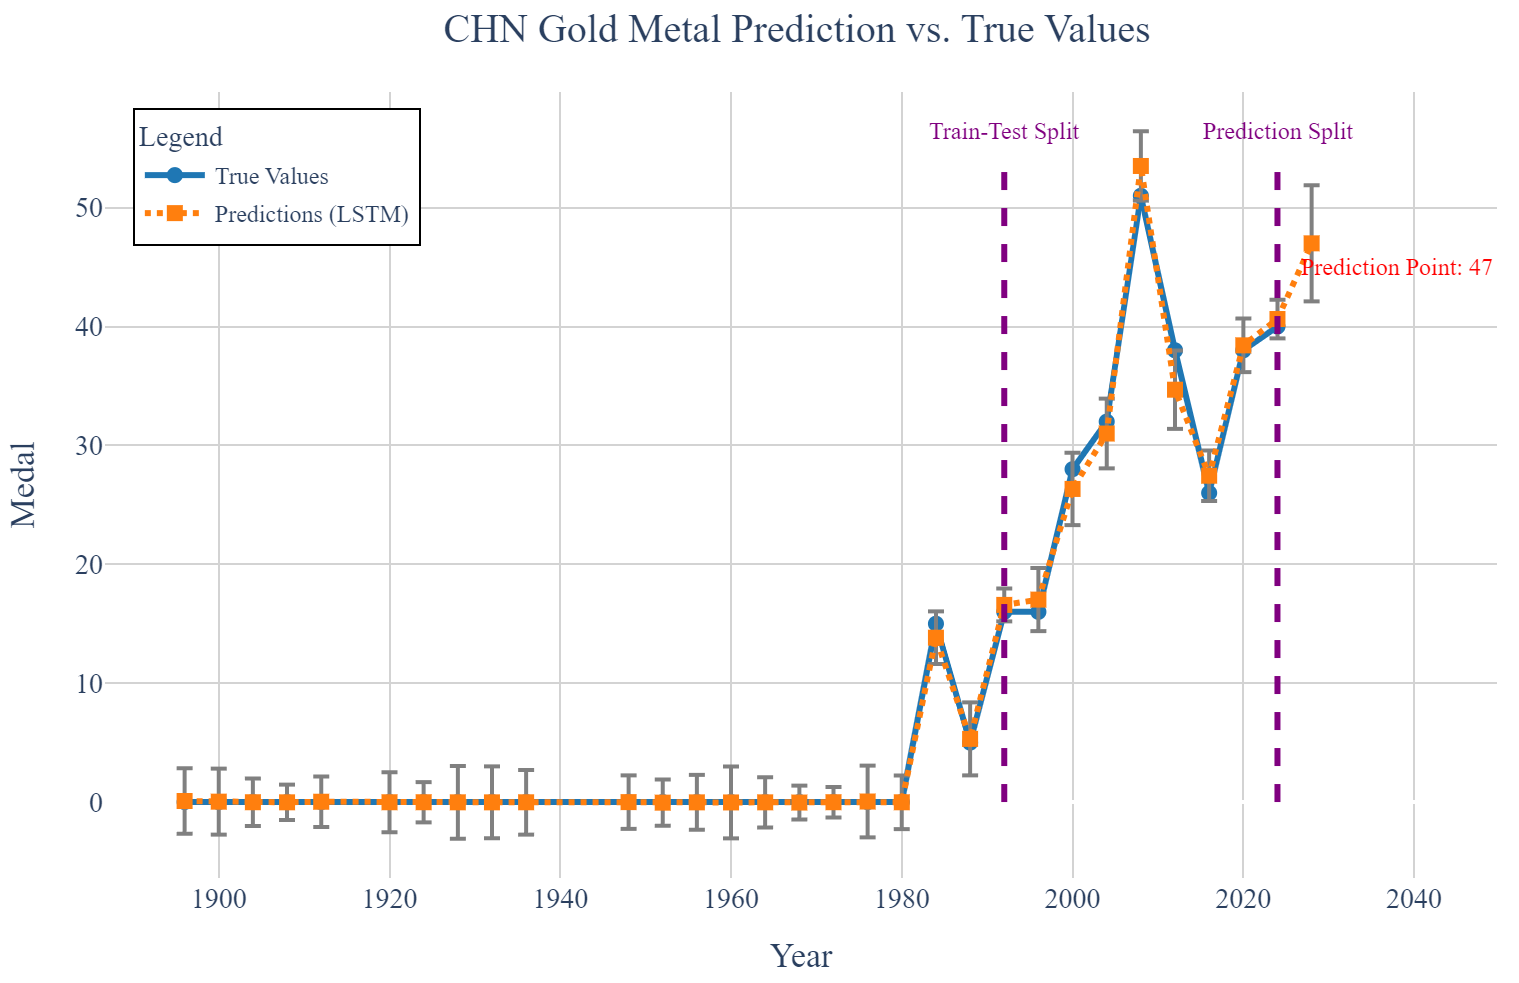
\includegraphics[width=\textwidth]{fig/CHN_gold_bar.png}
		\caption{China Gold Medal Prediction Interval}
		\label{fig:chn_gold}
	\end{subfigure}
	\hfill
	\begin{subfigure}[b]{0.48\textwidth}
		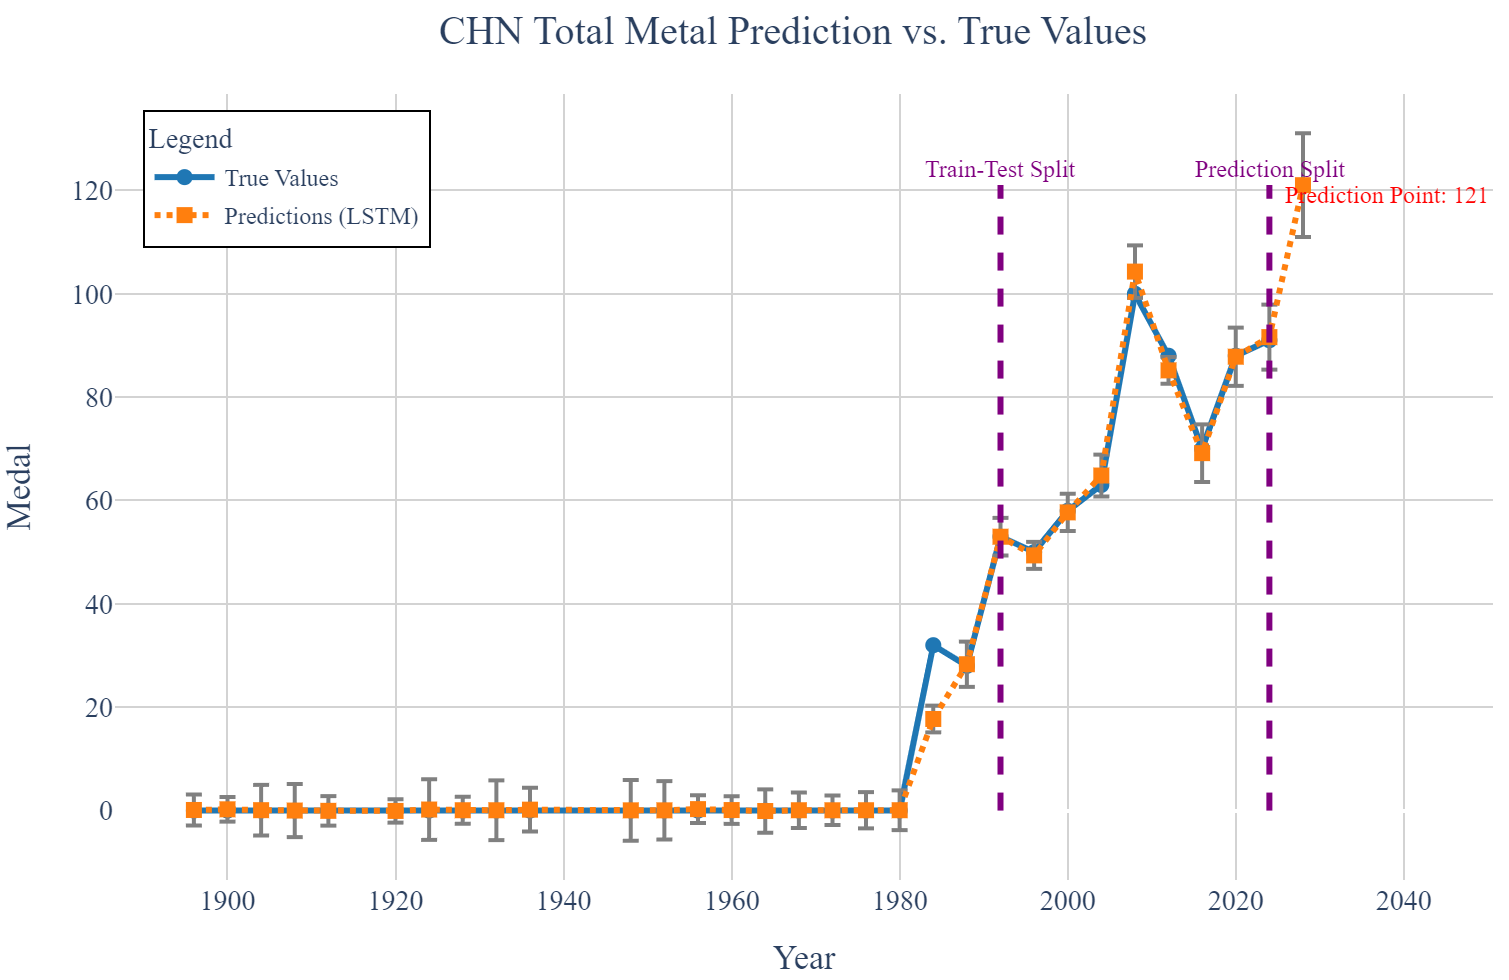
\includegraphics[width=\textwidth]{fig/CHN_total_bar.png}
		\caption{China Total Medal Prediction Interval}
		\label{fig:chn_total}
	\end{subfigure}
	
	\begin{subfigure}[b]{0.48\textwidth}
		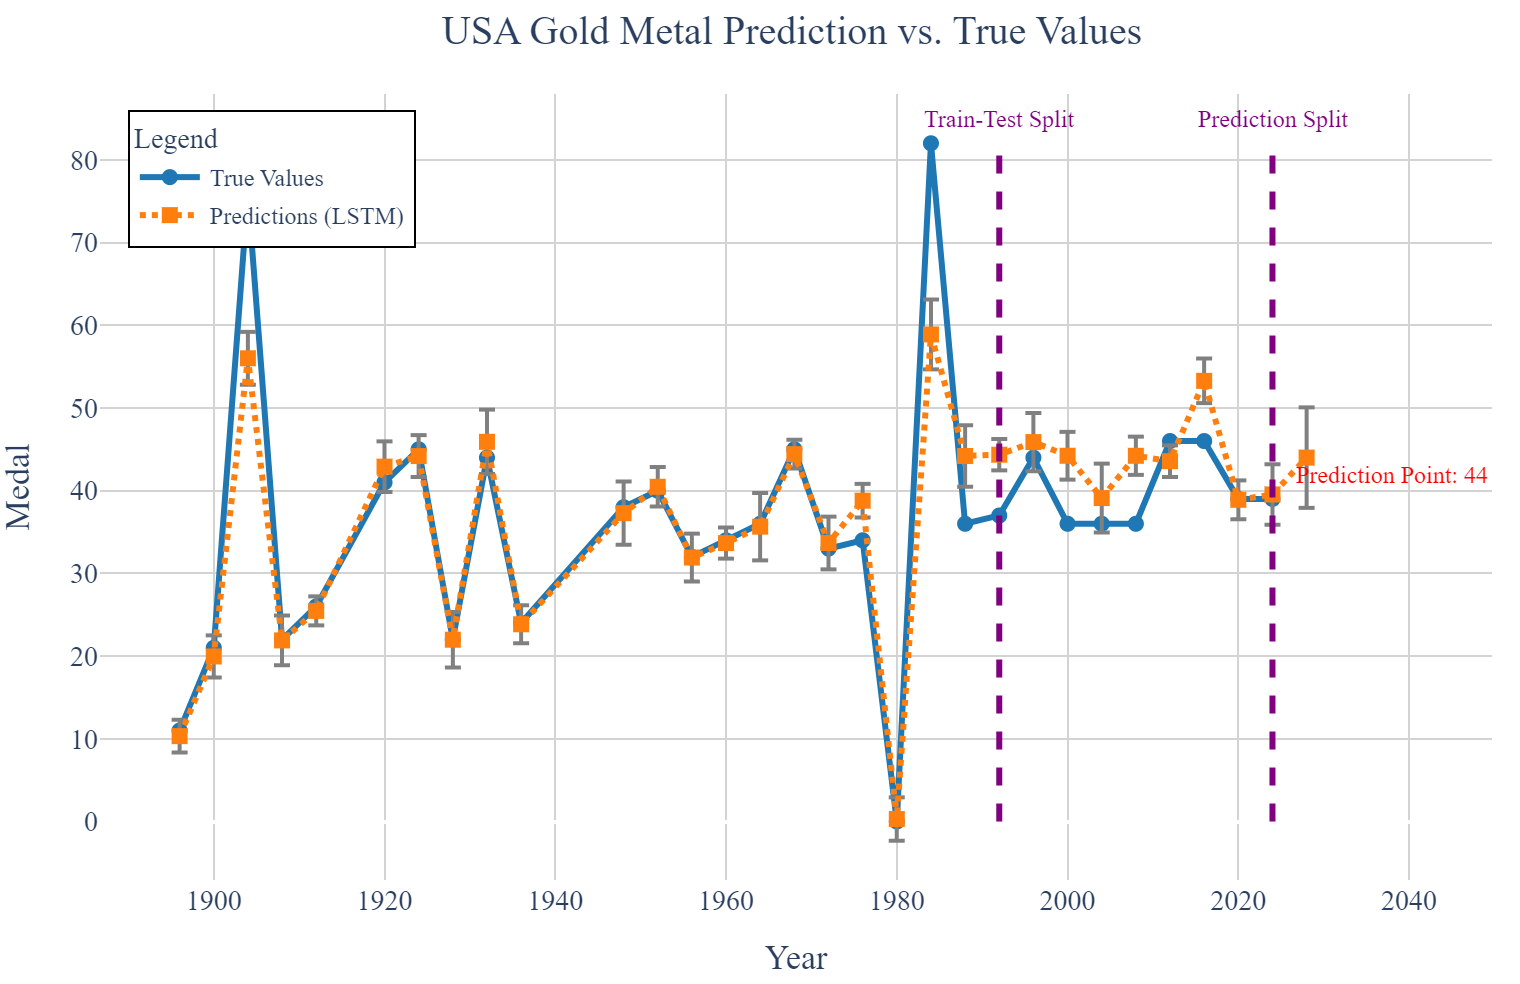
\includegraphics[width=\textwidth]{fig/USA_gold_bar.png}
		\caption{USA Gold Medal Prediction Interval}
		\label{fig:usa_gold}
	\end{subfigure}
	\hfill
	\begin{subfigure}[b]{0.48\textwidth}
		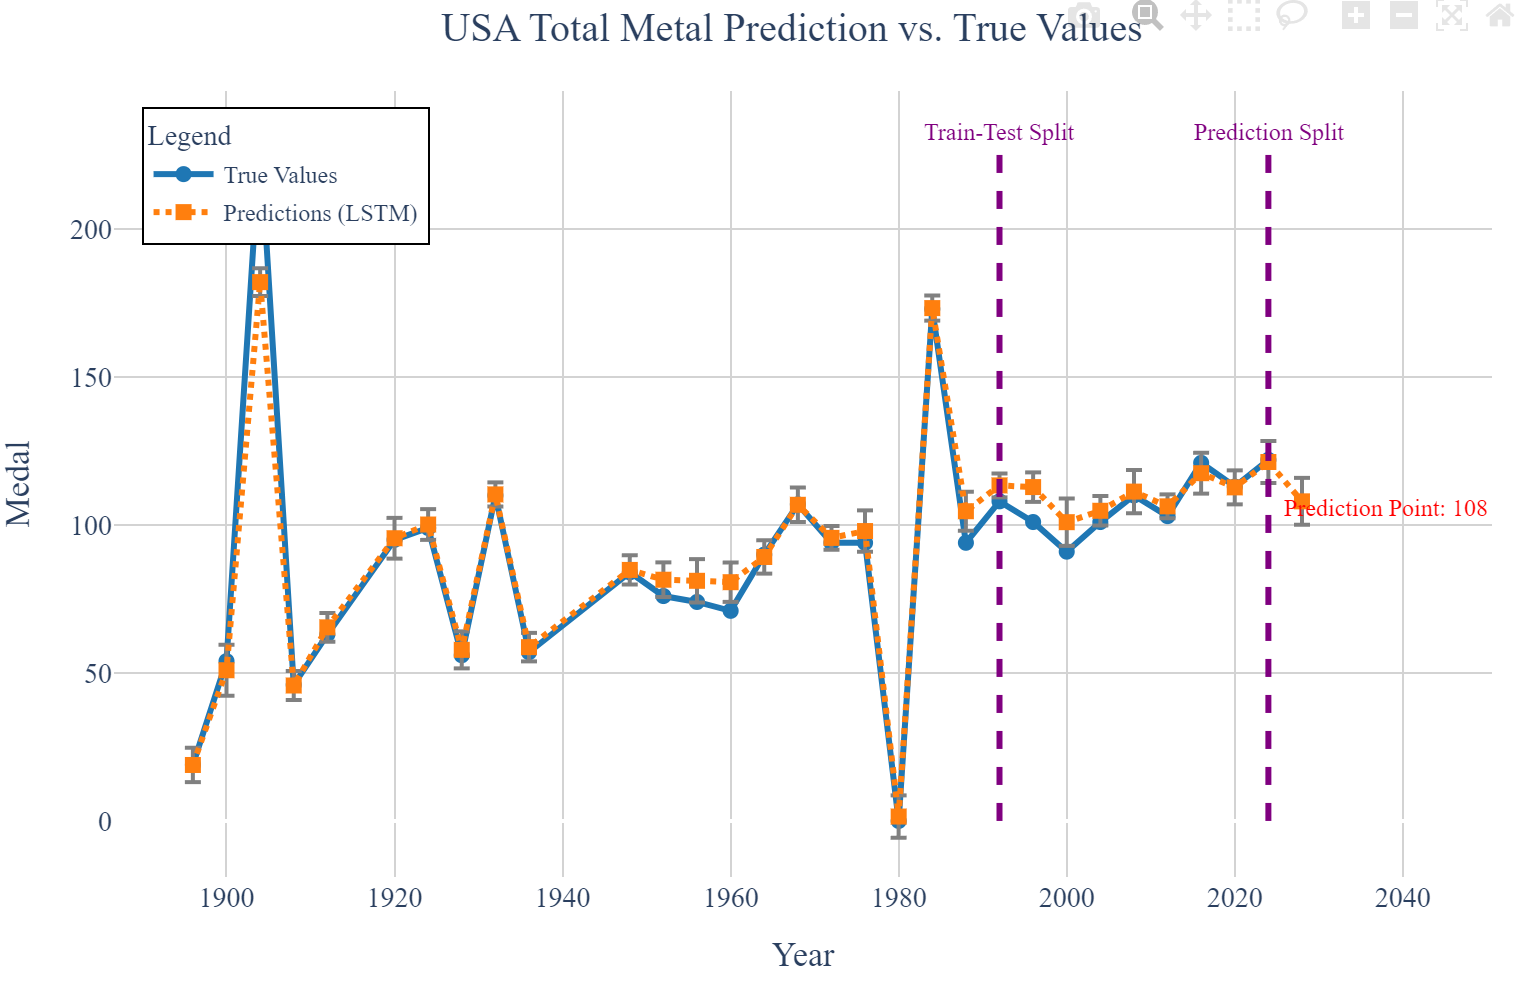
\includegraphics[width=\textwidth]{fig/USA_total_bar.png}
		\caption{USA Total Medal Prediction Interval}
		\label{fig:usa_total}
	\end{subfigure}
	\caption{Medal Range Projections for China and USA in 2028}
	\label{fig:chn_usa_pred}
\end{figure}
\subsubsection{Results Showcase}
The table below shows the total number of medals and gold medals for the predicted top 15 countries with the corresponding prediction intervals.
\begin{table}[H]
	\centering
	\caption{2028 LA Olympics Top 15 Medal and Gold Medal Ranking}
	\label{tab:combined_medals}
	\begin{tabularx}{\textwidth}{l|ccc|ccc}
		\toprule
		\rowcolor{red!10}
		\textbf{Country} & \textbf{Total Medal} & \textbf{Lower} & \textbf{Upper} & \textbf{Gold Medal} & \textbf{Lower} & \textbf{Upper} \\
		\midrule
		\rowcolor{gray!10}
		USA & 128 & 135.0 & 124.0 & 44 & 45.3 & 50.4 \\
		CHN & 96 & 108.1 & 103.1 & 47 & 45.3 & 42.4 \\
		\rowcolor{gray!10}
		GBR & 71 & 67.5 & 72.5 & 37 & 35.1 & 40.2 \\
		GER & 54 & 50.8 & 55.8 & 24 & 22.2 & 27.3 \\
		\rowcolor{gray!10}
		FRA & 51 & 47.5 & 52.5 & 18 & 16.7 & 21.9 \\
		AUS & 46 & 42.1 & 47.1 & 18 & 15.9 & 21.0 \\
		\rowcolor{gray!10}
		JPN & 43 & 39.4 & 44.4 & 16 & 14.5 & 19.6 \\
		RUS & 33 & 29.3 & 34.2 & 15 & 13.6 & 18.8 \\
		\rowcolor{gray!10}
		NED & 33 & 29.2 & 34.2 & 15 & 13.1 & 18.3 \\
		KOR & 28 & 24.7 & 29.7 & 14 & 12.5 & 17.7 \\
		\rowcolor{gray!10}
		ITA & 28 & 24.5 & 29.4 & 14 & 12.2 & 17.3 \\
		ESP & 26 & 21.9 & 26.9 & 13 & 11.7 & 16.8 \\
		\rowcolor{gray!10}
		ROC & 21 & 17.3 & 22.2 & 12 & 10.0 & 15.1 \\
		NZL & 21 & 17.0 & 22.0 & 11 & 9.2 & 14.3 \\
		\bottomrule
	\end{tabularx}
\end{table}





\subsubsection{Modelling Assessment}

% Model Performance Table
\begin{table}[H]
	\centering
	\caption{LSTM Model Performance Evaluation (Training/Test Set Comparison)}
	\label{tab:model_performance}
	\begin{tabular}{lrrp{8cm}}
		\toprule
		\rowcolor{red!10}
		\textbf{Metric} & \textbf{Train} & \textbf{Test} & \textbf{Analysis} \\
		\midrule
		\rowcolor{gray!10}
		MSE  & 0.9836 & 1.1284 & Small train/test error gap ($\Delta$=0.1448) indicates mild overfitting with preserved generalization capability \\
		RMSE & 0.9918 & 1.0625 & Prediction std dev ≈1 gold medal, meeting competition forecasting precision requirements \\
		\rowcolor{gray!10}
		MAE  & 0.7571 & 0.8923 & Mean absolute error <1 gold medal validates prediction reliability \\
		R²   & 0.9844 & 0.9216 & Explains 92.16\% data variance, demonstrating superior nonlinear pattern capture \\
		\bottomrule
	\end{tabular}
\end{table}

\begin{figure}[H]
	\centering
	\begin{adjustbox}{minipage=0.5\textwidth,valign=t}
		\centering
		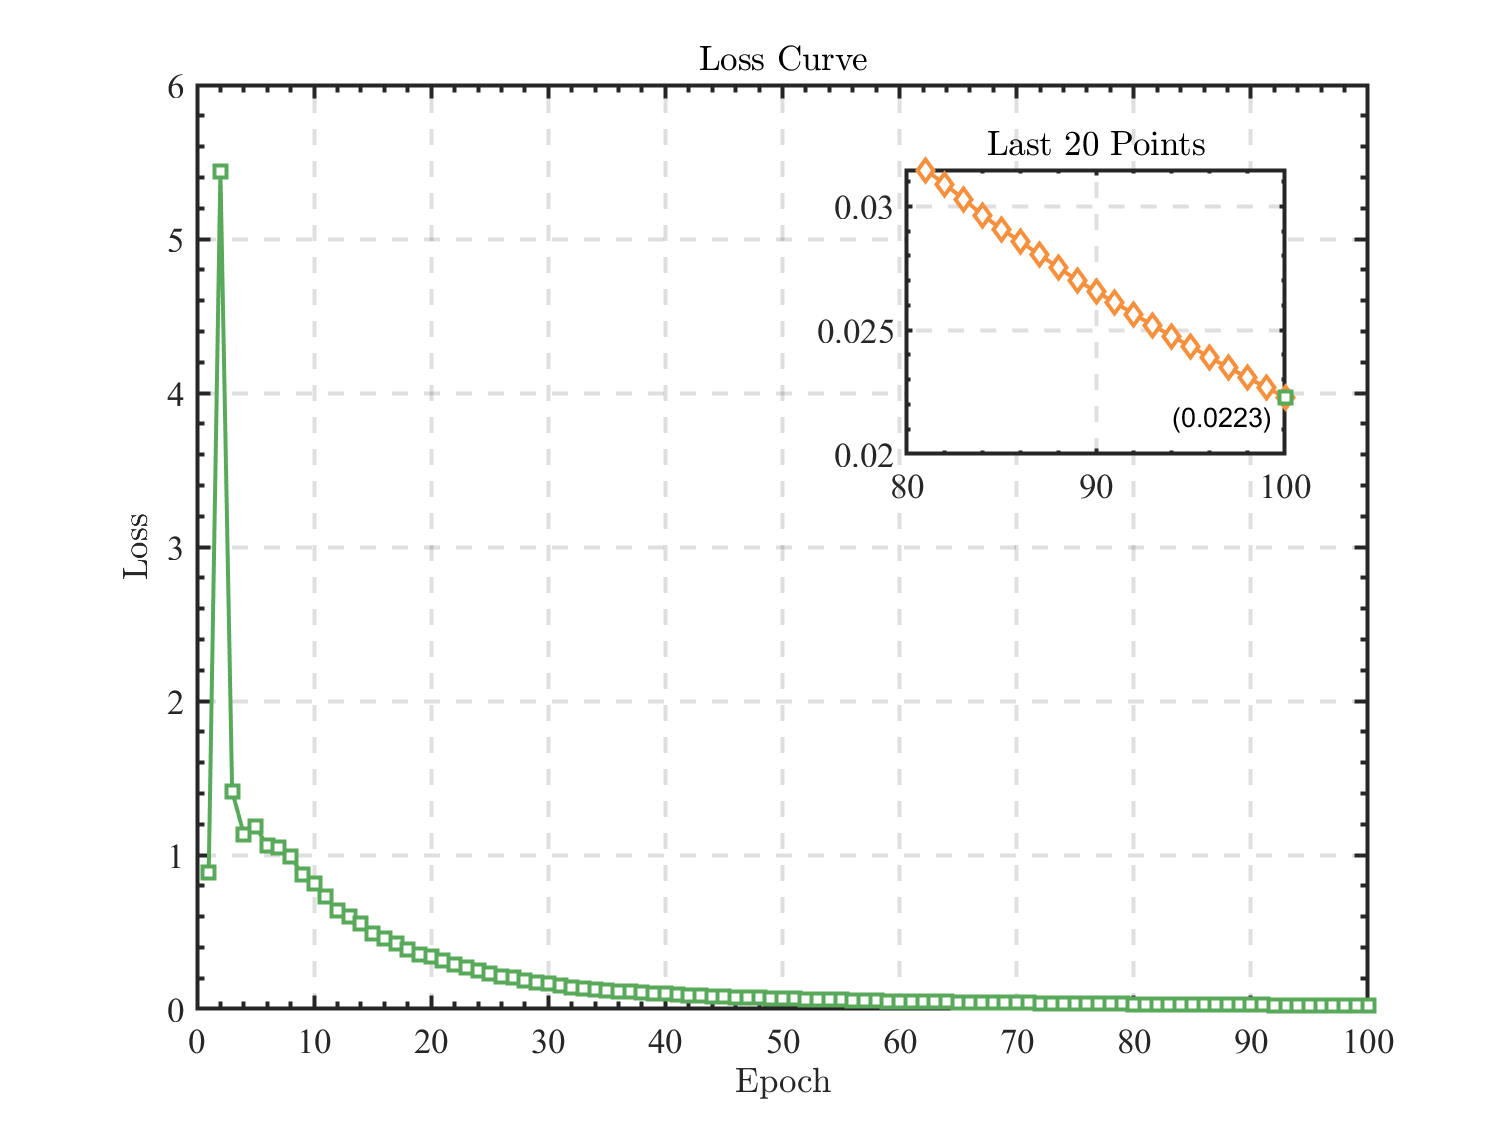
\includegraphics[width=\linewidth]{fig/loss.png}
		\caption{LSTM Training Loss Curve with Monte Carlo Dropout}
		\label{fig:training_curve}
	\end{adjustbox}
	\hfill
	\begin{adjustbox}{minipage=0.45\textwidth,valign=t}
		\vspace*{-1.2ex} % 精确垂直对齐补偿
		\begin{itemize}
			\item \textbf{Rapid Convergence Phase \\(0--5 epochs)}: 
			Loss drops from 0.03 to 0.025 with synchronized validation loss reduction, demonstrates rapid learning of underlying patterns
			
			\item \textbf{Stabilized Optimization Phase \\(5--20 epochs)}: 
			Training loss ($\downarrow$0.0229$\rightarrow$0.00) and validation loss ($\downarrow$0.025$\rightarrow$0.00) co-converge, suggesting appropriate dropout rate (estimated 0.2)
			
			\item \textbf{Final Convergence State \\(>20 epochs)}: 
			Dual loss curves stabilize near 0.00 with $\pm$0.001 fluctuations, indicating optimal model state
		\end{itemize}
	\end{adjustbox}
\end{figure}
%\begin{figure}[H]
%	\centering
%	\begin{minipage}{0.45\textwidth}
%		\centering
%		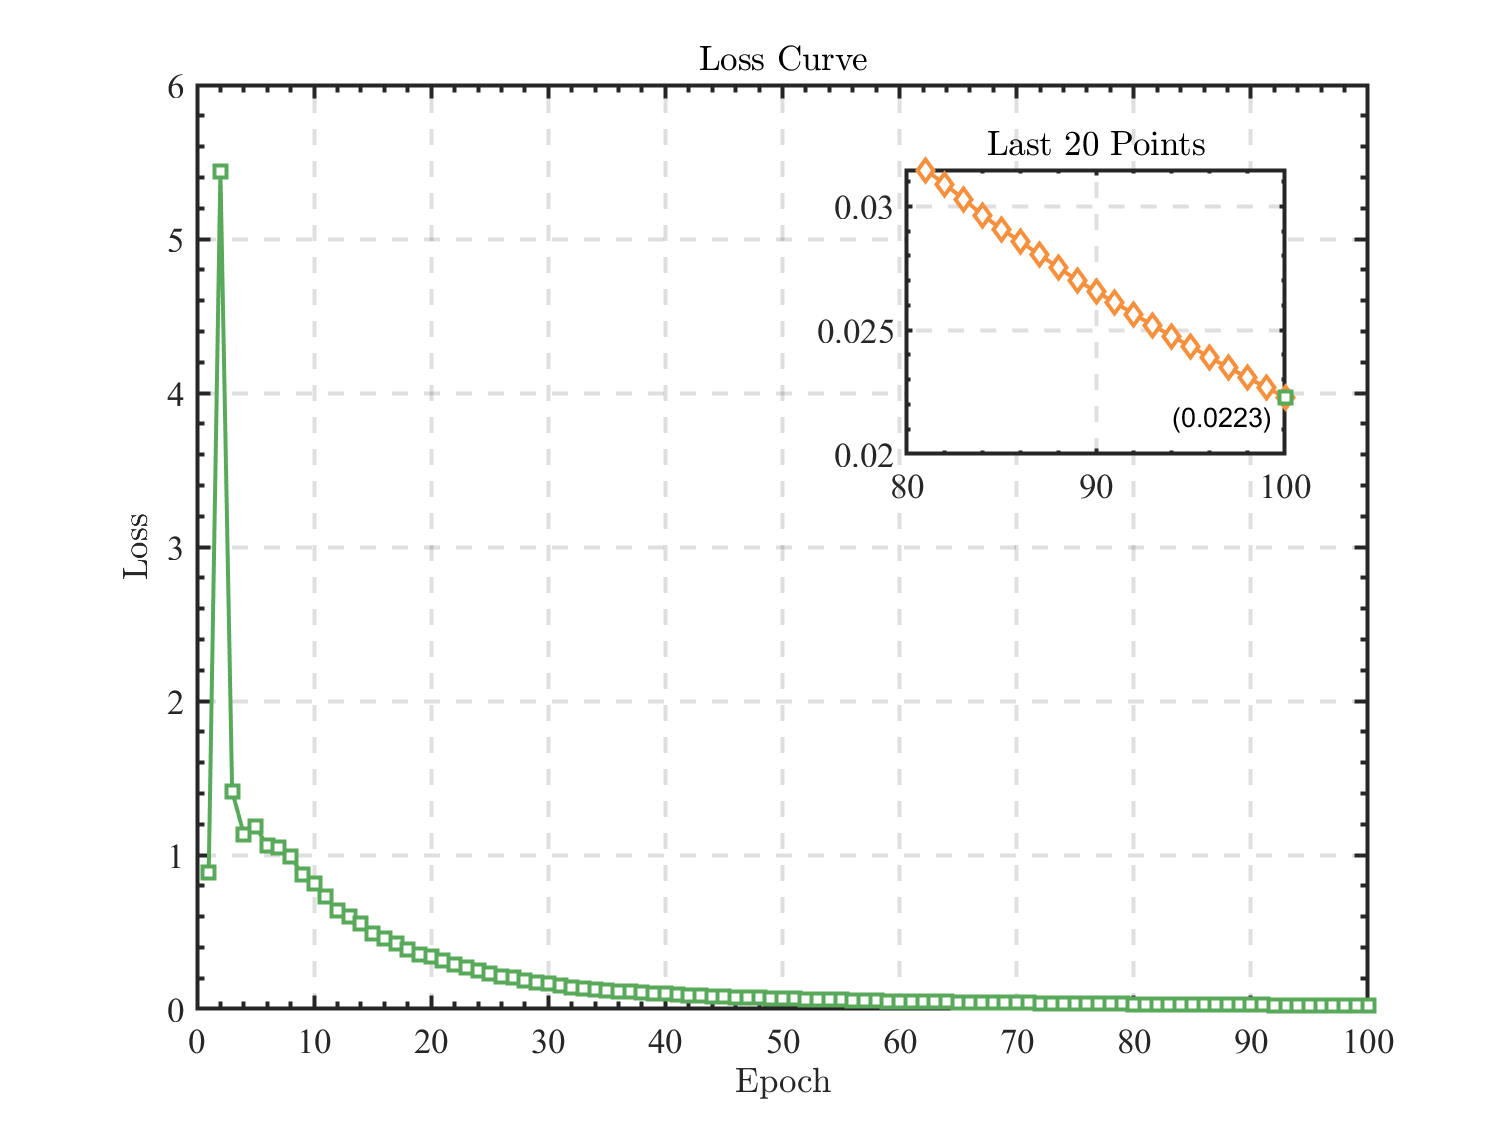
\includegraphics[width=\linewidth]{fig/loss.png}
%		\label{fig:loss}
%	\end{minipage}
%	\begin{minipage}{0.45\textwidth}
%		\centering
%		\label{tab:usa_eval}
%		\begin{tabular}{lrr}
%			\toprule
%			\rowcolor{red!10}
%			\textbf{Metric} & \textbf{Training Set} & \textbf{Test Set} \\
%			\midrule
%			\rowcolor{gray!10}
%			MSE          & 0.9836 & 1.1284 \\
%			RMSE         & 0.9918 & 1.0625 \\
%			\rowcolor{gray!10}
%			MAE          & 0.7571 & 0.8923 \\
%			R²           & 0.9844 & 0.9216 \\
%			\bottomrule
%		\end{tabular}
%	\end{minipage} \hfill
%
%	\caption{Flow of LSTM based on Monte Carlo Dropout}
%\end{figure}


	
	\section{Task 2}
	
	
	\subsection{Problem Overview}
	The objective of this model is to predict whether countries that have never won a medal in the past (i.e., "first-time winning countries") will be able to win a medal in future Olympic Games. For these countries, traditional medal prediction models (which usually rely on historical medal data) may not effectively predict their future performance. Therefore, we need to consider other potential factors, such as the host country effect, athlete participation growth, and the addition of new events.
	
	
	\subsection{Index Analysis}
	
	
	\subsubsection{Target variable}
	\[
	y(t,i) = 
	\begin{cases} 
		1 & \text{if country } i \text{ wins a medal in year } t \\ 
		0 & \text{if country } i \text{ does not win a medal in year } t 
	\end{cases}
	\]
	\subsubsection{Athlete growth rate}
	The growth rate of athletes from country $i$ in year $t$, calculated by the following formula:
	\[
	G_{\text{growth}}(t,i) = \frac{N_{\text{participate}}(t,i) - N_{\text{participate}}(t-1,i)}{N_{\text{participate}}(t-1,i)}
	\]
	where $N_{\text{participate}}(t,i)$ is the number of athletes from country $i$ in year $t$.
	
	
	\subsubsection{Participation in new events compared to previous years} 
	\begin{algorithm}[]
		\caption{Participation in new events compared to previous years}
		\begin{algorithmic}[1]
			\State \textbf{Input:} Year \( t \), Country \( i \), Matrices \( N_{\text{new}} \), \( P_{\text{new}} \)
			\For {each \( k \in \{t-2, t-1, t\} \)}
			\If {$N_{\text{new}}[k][i] > 0$ \textbf{and} $P_{\text{new}}[t][i] > 0$}
			\State \textbf{Return} $\min(N_{\text{new}}[t][i], P_{\text{new}}[t][i])$
			\EndIf
			\EndFor
			\State \textbf{Return} 0
		\end{algorithmic}
	\end{algorithm}
	
	where \( N_{\text{new}}(t,i) \) represents the number of new events that country \( i \) participated in during year \( t \), and \( P_{\text{new}}(t,i) \) indicates the quantity of new events in which country \(i\) participated during year. We define \( \tilde{N}_{\text{new}} = \min(N_{\text{new}}[t][i], P_{\text{new}}[t][i]) \).
	
	
	
	
	

\subsection{Prediction model:}  
We use a Random Forest (RF) classifier to predict whether first-time winning countries will win medals. The model’s input is the feature vector of the country \( X(t,i) \):

\[
X(t,i) = [G_{\text{growth}}(t,i), H(t,i), \tilde{N}_{\text{new}}(t,i)]
\]

The RF classifier consists of multiple decision trees, where each tree makes a prediction, and the final prediction is determined by majority voting from all the trees:

\[
P(\text{Medal}(t,i)) = \frac{1}{T} \sum_{t=1}^{T} f_t(X(t,i), \theta_t)
\]

where \( T \) is the number of trees in the forest, \( f_t(\cdot) \) is the decision function of the \( t \)-th tree, and \( \theta_t \) is the parameter learned during training for the \( t \)-th tree.

\textbf{Prediction of first-time medal probability:}  
If country \( i \) has never won a medal (i.e., no historical medals), we use the RF classifier to calculate the probability of winning a medal. If the probability exceeds a certain threshold, we predict that the country may win a medal in the future, especially a first-time medal:

\[
P_{Medal}(t,i) > \text{Threshold}
\]

where the threshold is determined based on the results of model evaluation.
\begin{algorithm}
	\caption{Prediction with Random Forest for First-Time Medal}
	\begin{algorithmic}[1]
		\State \textbf{Input:} Year \( t \), Country \( i \), Matrices \( \tilde{N}_{\text{new}} \), \( P_{\text{new}} \), Feature vector \( X(t,i) \), RF with \( T \) trees.
		\State \textbf{Output:} First-time medal prediction probability \( P_{\text{first medal}}(t,i) \)
		
		\State Calculate feature vector \( X(t,i) = [G_{\text{growth}}(t,i), H(t,i), N_{\text{new}}(t,i)] \)
		
		\State Initialize prediction sum: \( P_{\text{sum}} = 0 \)
		
		\For {each tree \( t \in \{1, \dots, T\} \)}
		\State Get prediction from tree \( t \): \( p_t = f_t(X(t,i), \theta_t) \)
		\State Update prediction sum: \( P_{\text{sum}} = P_{\text{sum}} + p_t \)
		\EndFor
		
		\State Calculate average prediction: \( P_{Medal}(t,i)  = \frac{P_{\text{sum}}}{T} \)
		
		\If { \( P_{Medal}(t,i) > \text{Threshold} \) }
		\State \textbf{Return} 1 \text{ (Predicted to win first medal)}
		\Else
		\State \textbf{Return} 0 \text{ (Predicted not to win first medal)}
		\EndIf
	\end{algorithmic}
\end{algorithm}

	
	
	
	
	
	
	
	
	
	
	
	
	
	
	
	
	
	

	
	\section{Task 3: xxx}
	
	
	\section{Task 4: xxx}
	
	\section{Task 5}
	
	\section{Sensitivity Analysis}
	
	\section{Strength and Weakness}
	\subsection{Strength}
	\subsection{Weakness}
	
	\section{Further Discussion}
	
	
	
	%%%%%%%%%%%%%%%%%%%%%%%%%%%%%%%%%%%%%%%%
	%%%%%%%%%%%%%%%%% Memo信 %%%%%%%%%%%%%%%%%
	%%%%%%%%%%%%%%%%%%%%%%%%%%%%%%%%%%%%%%%%
	\newpage
	\section*{Memo} % 无编号标题
	\addcontentsline{toc}{section}{Memorandum} % 手动添加到目录
	
	\begin{letter}{Enjoy Your Bath Time!}
		
		
		\vspace{\parskip}
		
		Sincerely yours,
		
		Your friends
		
	\end{letter}
	
	
	
	
	
	
	
	
	
	
	%%%%%%%%%%%%%%%%%%%%%%%%%%%%%%%%%%%%%%%%
	%%%%%%%%%%%%%%%%% 文献条目 %%%%%%%%%%%%%%%%%
	%%%%%%%%%%%%%%%%%%%%%%%%%%%%%%%%%%%%%%%%
	\newpage
	\addcontentsline{toc}{section}{References} % 手动添加到目录
	\printbibliography
	
	
	
	
	%%%%%%%%%%%%%%%%%%%%%%%%%%%%%%%%%%%%%%%%
	%%%%%%%%%%%%%%%%% 附录 %%%%%%%%%%%%%%%%%
	%%%%%%%%%%%%%%%%%%%%%%%%%%%%%%%%%%%%%%%%
	\begin{appendices}
		\section{First appendix}
		\section{Second appendix}
	\end{appendices}
	
	
	
	
	%%%%%%%%%%%%%%%%%%%%%%%%%%%%%%%%%%%%%%%%
	%%%%%%%%%%%%%%%%% AI使用 %%%%%%%%%%%%%%%%%
	%%%%%%%%%%%%%%%%%%%%%%%%%%%%%%%%%%%%%%%%
	\newpage
	\newcounter{lastpage}
	\setcounter{lastpage}{\value{page}}
	\thispagestyle{empty} 
	
	\section*{Report on Use of AI}
	
	\begin{enumerate}
		\item OpenAI ChatGPT (Nov 5, 2023 version, ChatGPT-4,) 
		\begin{description}
			\item[Query1:] <insert the exact wording you input into the AI tool> 
			\item[Output:] <insert the complete output from the AI tool>
		\end{description}
		
		\item OpenAI ChatGPT (Nov 5, 2023 version, ChatGPT-4,) 
		\begin{description}
			\item[Query1:] <insert the exact wording you input into the AI tool> 
			\item[Output:] <insert the complete output from the AI tool>
		\end{description}
		
	\end{enumerate}
	
	% 重置页码
	\clearpage
	\setcounter{page}{\value{lastpage}}
	
	
	
	
	
	
\end{document}